\documentclass{ieeeaccess}
\usepackage{cite}
\usepackage{amsmath,amssymb,amsfonts}
\usepackage{algorithmic}
\usepackage{graphicx}
\usepackage{textcomp}

\usepackage{fancyvrb}
%\usepackage{caption}
\usepackage[utf8]{inputenc}

\pdfminorversion=4

\def\BibTeX{{\rm B\kern-.05em{\sc i\kern-.025em b}\kern-.08em
    T\kern-.1667em\lower.7ex\hbox{E}\kern-.125emX}}
\begin{document}
\history{Date of publication xxxx 00, 0000, date of current version xxxx 00, 0000.}
\doi{10.1109/ACCESS.2017.DOI}

\title{Integration of Anonymous Credential Systems in IoT constrained environments}
\author{\uppercase{Jose Luis Canovas Sanchez},
\uppercase{Jorge Bernal Bernabe, and Antonio F. Skarmeta}
}
\address{Department of Information and Communications Engineering\\
	Computer Science Faculty, 
	University of Murcia, Spain\\
	\{joseluiscanovas, jorgebernal, skarmeta\}@um.es\\
}
%\address[1]{National Institute of Standards and 
%Technology, Boulder, CO 80305 USA (e-mail: author@boulder.nist.gov)}
%\address[2]{Department of Physics, Colorado State University, Fort Collins, 
%CO 80523 USA (e-mail: author@lamar.colostate.edu)}
%\address[3]{Electrical Engineering Department, University of Colorado, Boulder, CO 
%80309 USA}
\tfootnote{This work has received funding from IBM 2015 Faculty Award for Cyber Security and the European Union’s Horizon 2020 research and innovation programme under grant agreement No 700085 (ARIES project).}

\markboth
{Author \headeretal: Preparation of Papers for IEEE TRANSACTIONS and JOURNALS}
{Author \headeretal: Preparation of Papers for IEEE TRANSACTIONS and JOURNALS}

%\corresp{Corresponding author: First A. Author (e-mail: author@ boulder.nist.gov).}

\begin{abstract}
The pervasive nature of Internet of Things entails additional threats that compromise the security and privacy of IoT devices and, eventually, the users. This issue is aggravated in constrained IoT devices equipped with minimal hardware resources. Current security and privacy implementations need to be re-designed and implemented maintaining its Level of Assurance (LoA), aiming for this family of devices. To cope with this issue, this paper proposes the first novel attempt to leverage Anonymous Credential Systems (ACS) to preserve the privacy of autonomous IoT constrained devices. Concretely, we have designed a solution to integrate IBM's Identity Mixer into constrained IoT ecosystems, endowing the IoT with ACS's privacy-preserving capabilities. The solution has been designed, implemented and evaluated proving its feasibility.
\end{abstract}

\begin{keywords}
Anonymous credential system, Identity Mixer, Internet of Things, Zero-knowledge proof
\end{keywords}

\titlepgskip=-15pt

\maketitle


\section{Introduction}

Internet of Things is a term with a wide range of interpretations \cite{Atzori20102787}, breafly, we can think of it as billions of devices, mainly resource constrained, which are interconnected between them and the Internet, in order to achieve a goal.

Many of this objectives require the use of a great amount of data, and thanks to organizations like WikiLeaks, people are aware of the implications of their data on the Internet, demanding more security and privacy for it. This includes not only the data shared with others, where one must trust they will keep it safe, but it is also the data collected about us and which we do not have direct control over it.

In traditional M2M (Machine to Machine) environments the issues about security and privacy have already been treated deeply, but in the IoT ecosystem, due to it's recent and fast growth, it lacks of those tools to autonomously solve these issues.

To address these problems of privacy in the Internet, a recent approach is the concept of \textit{strong anonymity}, that conceals our personal details while letting us continue to operate online as a clearly defined individuals \cite{stronganonymity}. To achieve it, we must address a way to perform authentication and authorization in the most privacy-friendly approach. Anonymous credentials and selective disclosure techniques allow us to control what information we reveal to others.

The most common type of ACS are ABCs (Attribute-Based Credentials), which can be thought of as a digital signature by an Issuer on a list of attribute-value pairs \cite{introCredIBM}.
The most straightforward way for a user to convince a Verifier of her list of attributes would be to simply transmit her credential to the Verifier.
With anonymous credentials, the user never transmits the credential itself, but rather uses it to convince the Verifier that her attributes satisfy certain properties - without leaking any information about the credential other than the chosen properties to display. 
Stronger even, apart from showing the exact value of an attribute, the user can even convince the
Verifier that some complex predicate over the attributes holds, e.g. that her birth date was more than 18 years ago, without revealing the real date.

With classical symmetric and asymmetric cryptography it seems rather impossible to create such credentials without an explosion of signatures over every possible combination of attributes. For this reason, current solutions rely on  Zero-Knowledge Proofs (ZKP), cryptographic methods that allow to proof knowledge of some data without disclosing it.

Based on ZKPs, IBM developed Identity Mixer\footnote{Identity Mixer - \url{https://www.zurich.ibm.com/identity_mixer/}}, %broken url
Idemix for short, a protocol suite for privacy-preserving authentication and transfer of certified attributes. It allows user authentication without divulging any personal data. Users have a personal certificate with multiple attributes, but they can choose how many to disclose, or only give a proof based on their values. Thus, no personal data is collected that needs to be protected, managed, and treated by third parties.

So far, Idemix or privacy-ABCs have been successfully applied to deal with traditional Internet scenarios, in which users can authenticate and prove their attributes against a service provider. However, due to the reduced computational capabilities of certain IoT devices, it has not been yet considered for IoT scenarios. As it is presented in the state of the art chapter, current implementations of Idemix are based on Java, which requires high computational and memory resources to be executed, and to the best of our knowledge, this is the first proposal that tries to apply an IoT solution for privacy-preserving authentication and authorization, based on Anonymous Credential Systems.

The design and implementation presented in this paper will allow constrained IoT devices to carry out all actions available in the Idemix protocol, being in control of the decisions to take in every step. This achieves oblivious interactions between any traditional machine using Idemix and the IoT devices, without having to adapt the protocol, or a subset it, to interact with these new entities.

\hfil

This document is structured as follows: Section \ref{ch:stateoftheart} provides a state of the art analysis through the history of Idemix and related works, analysing what is of the most interest for the IoT perspective. Section \ref{ch:design} presents a formal design of the proposed IoT and Idemix solution. Section \ref{ch:implementation} describes the PoC implementation developed. After any implementation, it is a must to validate it, as showed during the performance tests in section \ref{ch:validation}. Finally, our conclusions and lines for future work are described in section \ref{ch:conclusions}.



\section{State of the art}\label{ch:stateoftheart}

In this section we present a showcase of competing ACS solutions, focusing their application for the IoT, where the two most notable alternatives to Idemix are Persiano's ABC systems and Microsoft's U-Prove.

%%%%%%%%%%%%%%%%%%%%%%%%


In 2004, Persiano and Visconti presented a non-transferable anonymous
credential system that is multi-show and for which it is possible to prove
properties (encoded by a linear Boolean formula) of the credentials \cite{Persiano2004}. Unfortunately, their proof system is not efficient since the step in which a user proves possession of credentials (that needs a number of modular exponentiations that is linear in the number of credentials) must be repeated $k$ times (where $k$ is the security parameter) in order to obtain a satisfying soundness.

%%%%%%%%%%%%%%%%%%%%%%%%%

Based on Persiano's proofs, an anonymous authentication for privacy-preserving IoT was presented in \cite{alcaide2013anonymous}, but the studied performance analysis was carried out using Java on a traditional desktop PC, theoretically assuming IoT devices to be proportionally 40 times slower than the testing machine.


%%%%%%%%%


In 2000, Stefan Brands provided the first integral description of the U-Prove
technology in his thesis \cite{uprove}, after which he founded the company Credentica
in 2002 to implement and sell this technology. Microsoft acquired Credentica
in 2008 and published the U-Prove protocol specification \cite{uprove2} in 2010
under the Open Specification Promise4 together with open source reference software
development kits (SDKs) in C\# and Java.
The U-Prove technology is centered around a so-called U-Prove token. This
token serves as a pseudonym for the prover. It contains a number of attributes
which can be selectively disclosed to a verifier. Hence, the prover decides which
attributes to show and which to withhold. Finally there is the token’s public-key, which aggregates all information in the token, and a signature from the issuer
over this public-key to ensure the authenticity \cite{book:947508}.

%%%%%%%%%%%


\hfil

Independently of the mentioned technologies, Jan Camenisch, Markus Stadler and Anna Lysyanskaya studied in \cite{Camenisch:GroupSig,Camenisch:AnonCred,camenisch2002signature} 
the cryptographic bases for signature schemes and anonymous credentials that later became IBM's Identity Mixer protocol specification \cite{idemixSpec}.


Luuk Danes in 2007 studied theoretically how Idemix's User role could be implemented using  
smart cards \cite{luuk}, identifying what data and operations should be kept inside the device to perform different levels of security. The User role was divided between the smart card, holding secret keys, and the Idemix terminal, that commanded operations inside the smart card, or read the keys in it to perform the instructions itself. The studied sets were a combination of possibilities where the smart card would give all the information to the terminal, only partial information, or keep everything secret and perform all the private operations within itself.

Later, in 2008 V\'ictor Sucasas also studied an anonymous credential system with smart card support \cite{sucasas}, equivalent to a basic version of Idemix, using a simulator to test the PoC and pointing out some crucial implementation details for performance. The researching tendency starts to show that smart cards are the best solution to hold safely the User's credentials.

In 2009, some Java smart card PoC for Idemix were developed in \cite{javaIdemix1} and \cite{javaIdemix2}, but they weren't optimal and didn't include some Idemix's functionalities, like selective disclosure.

In 2013, Vullers and Alpar, implemented an efficient smart card for Idemix \cite{vullers2013efficient}, aiming to integrate it in the IRMA\footnote{The IRMA project has been recently included in the Privacy by Design Foundation: \url{https://privacybydesign.foundation/}} project, and comparing the performance with U-Prove's smart cards. This new implementation was written in C, under the MULTOS platform for smart cards, and describes many decisions made during the development to improve the performance on such constrained devices. The terminal application was written in Java and used an extension of the Idemix cryptographic library to take care of the smart card specifics.


Later, the P2ABCE\footnote{\url{https://github.com/p2abcengine/p2abcengine}} project extended the concept of smart cards, physical or logical, as holders of the credentials.  The P2ABCE project is a language framework that unifies different cryptographic ABC engines and policies, currently supporting U-Prove and Idemix. The Idemix library was updated to support P2ABCE and their last version is therefore interoperable with U-Prove. The smart card specification from the P2ABCE project can be considered the official version to work with. The Identity Mixer team instructs the use of P2ABCE in order to use Idemix itself.


Related to the IoT, the P2ABCE project has been used to test in a VANET\footnote{Vehicular Ad-Hoc Network} scenario how an OBU (On Board Unit) with constrained hardware could act as a User in a P2ABCE ecosystem \cite{vanet}. However, after the theoretical analysis, the paper only simulates a computer with similar performance as an OBU, without adapting the existing Java implementation of P2ABCE to a real VANET system.

Another recent approach to integrate Idemix in the IoT was performed in \cite{DBLP:journals/mis/BernabeRG17}, where it can be seen as a first attempt of a real re-implementation, not simulation, but aimed for Android devices, written in Java, and therefore, not suitable for constrained devices either.






\section{Design of the proposed solution}\label{ch:design}

This section describes the design of our proposal to integrate IoT constrained devices as part of the privacy preserving ecosystem P2ABCE. The ultimate goal is to enable constrained IoT devices to play the Idemix User and Verifier roles, interacting autonomously in order to authenticate and demonstrate their credential attributes to any Verifier in a privacy-preserving fashion, as well as verifying other devices in a M2M environment, addressing the power and memory constrains many IoT devices face. These requirements and objectives are structured below:

%When designing a privacy preserving solution for IoT, we must aim for a series of objectives that guarantee its integrity and usability. Our requirements are:

%\textbf{Solution requirements and objectives}

\begin{itemize}
	\item \textit{Security}: the solution should not compromise the security of the device's identities.
	\item \textit{Usability}: it should provide an API for developers to use the P2ABCE privacy capabilities in their applications.
	\item \textit{Full P2ABCE support}: the IoT device should be capable of performing every action a traditional User or Verifier could perform.
	\item \textit{Transparent interactions}: any third party actor of the system should not be aware of the IoT condition of the device, therefore, there should be no changes to the P2ABCE protocol.
	\item \textit{Constrained devices}: the solution should aim to be portable and applicable to as many IoT devices as possible, including those with less computing capabilities.
\end{itemize}

\hfil

To address these objectives, considering the evolution of Identity Mixer to use smart cards, our solution will consist on a mandatory implementation of the smart card logic inside the IoT device, which will conceal all the operations regarding secret keys, and to manage the P2ABCE language, the solution shall offer an API which, at the time being, will perform \textit{computation offloading} to a device capable of running the framework.

Even in the case all P2ABCE were to be implemented inside an IoT device, it should implement the support for software smart cards, to keep the secret inside the IoT device. Therefore, the first step is to implement the smart card logic inside the IoT device, and later, if the device resources admit it, other components of the P2ABCE framework.

Computation offloading is not a new technique for IoT environments. For example, to reduce the overhead of IPv6, 6LoWPAN compresses packets and uses smaller address sizes. In order to communicate a 6LoWPAN with other networks, the IoT devices delegate on a proxy that can manage the 6LoWPAN and IPv6 stacks. In the scope of consumer devices, smart watches can install applications which delegate on the user's phone to accomplish performance demanding task. 
Therefore, the IoT device now has a \textbf{duality} in its functions, because it is the User that starts any interaction with other actors, and it is also the smart card that a P2ABCE server must ask for cryptographic operations. It can also be seen as a \textbf{double delegation}. The IoT device delegates on the external P2ABCE server to manage the protocol, and that P2ABCE server delegates on the IoT device, acting now as the smart card.

Regarding the communication between different P2ABCE actors, it depends on each IoT scenario, independently of our solution, as third party actors have no need to adapt the P2ABCE protocol.



% TODO mencionar más adelante qué se ha conseguido de cada
% Security : el canal seguro y autenticado entre servidor y IoT, así como mantener la IoT smart card segura
% Usability : el toolkit permite al fabricante usarlo como una API y usar el despliegue que prefiera, actuando como recipient al inicio
% Full support & transparent : el parser se ejecuta en el servidor completo y se podría implementar en el dispositivo si la potencia lo permite
% Constrained : técnica de computation offloading

% TODO : escenarios de aplicación



To ensure that our solution does not risk the security of the device's secrets, the next section introduces the fundamentals on the operations performed by a User, therefore identifying the key operations to implement in the smart card.

\subsection{Fundamentals on Zero-Knowledge Proofs}

% Ejemplo de DL problem
% Firma CL
% Mostrar al final la estructura de la mayoría de ZKP : commitment(s), challenge, response(s)

To understand Zero-Knowledge Proofs, \textit{Fundamentals of Computer Security} \cite[Chapter 12]{book:856771} offers a good introduction to the topic. Here is shown how one can indeed proof knowledge of a value, without revealing it, using the classic ZKP of knowledge based on the discrete logarithm problem, also known as Schnorr's identification scheme. Based on this discrete logarithm ZKP, Idemix then derives multiple ZKPs of relations and properties of the values hidden in a credential.


Using the notation introduced by Camenisch and Stadler \cite{camenisch1997efficient}, the discrete logarithm ZKP can be written as 
\[ PK\{ (\alpha) : y = g^\alpha \}  \]
given a known group $G=\left\langle g \right\rangle $ of prime order $q$ and public value $y\in G$. The notation means: ``I know a secret value $\alpha$ such that $g^\alpha$ is $y$'', i.e. the discrete logarithm of $y$, $log_g y = \alpha$.


During the first step of the protocol, the prover chooses randomly a value $r_\alpha$, computes the \textit{commitment} $t := g^{t_\alpha}$ and sends $t$ to the verifier. 
Then, the verifier chooses another random exponent, the \textit{challenge} $c$, and sends it to the prover. 
Next, the prover computes the \textit{response} $s:=r-c\alpha\, mod\, q$ and sends it to the verifier.
Finally, the verifier checks whether or not $ t \overset{?}{=} g^{s_\alpha} y^c $ holds. The verifier never receives the secret value $\alpha$, and the verifier will not be able to compute it given $t$ and $s$.

The protocol holds because $ g^{s_\alpha} y^c  =  g^{r_\alpha - c\alpha} g^{\alpha c} = g^{r_\alpha} = t $.

\begin{figure}[bth]
	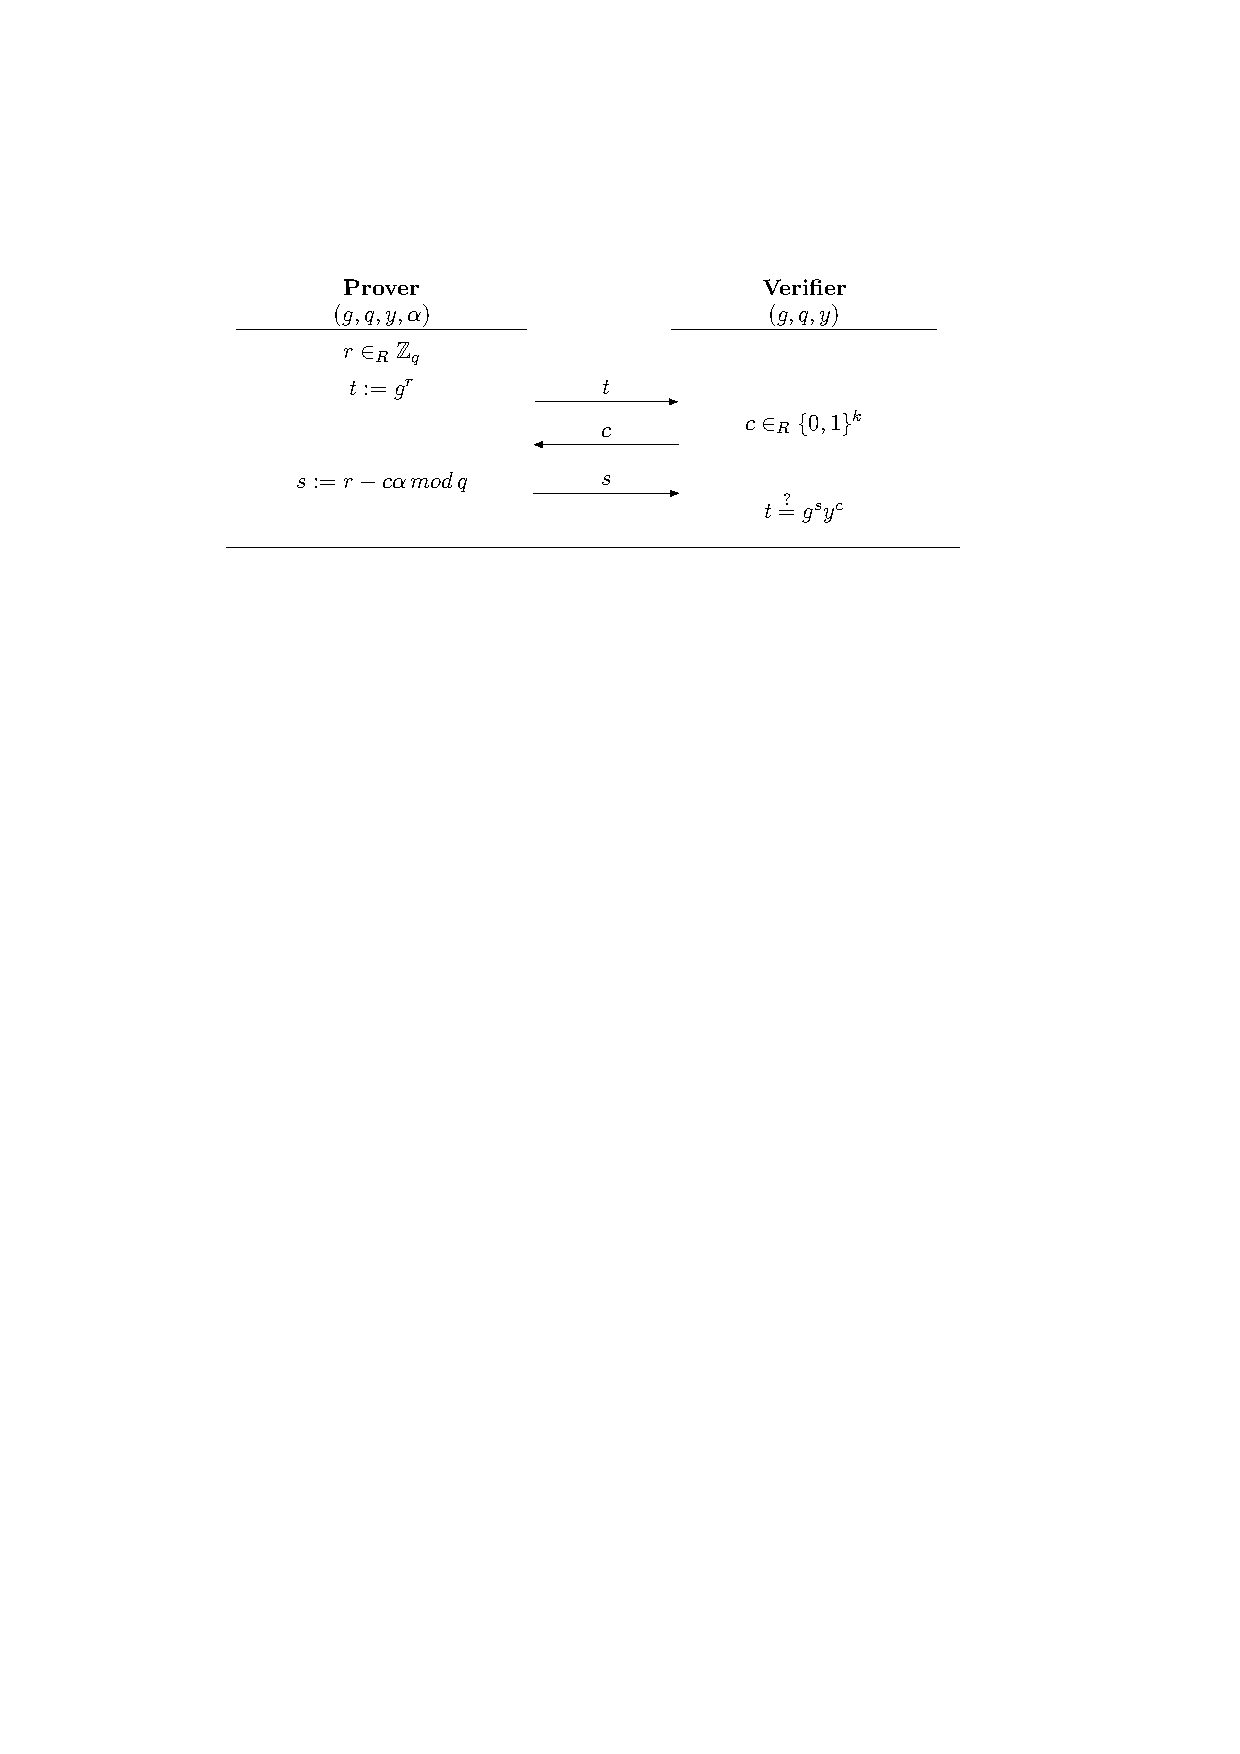
\includegraphics[width=\linewidth]{gfx/schnorr}
	\caption{Schnorr's protocol $PK\{ (\alpha) : y = g^\alpha \}$. The prover knows $(g,q,y,\alpha)$ such that $g^\alpha=y$. The verifier knows $(g,q,y)$.}
	\label{fig:schnorr}
\end{figure}

The Fiat-Shamir heuristic lets us replace the verifier challenge with a hash function $\mathcal{H}$, computing the challenge as $c:=\mathcal{H}(g\mid y\mid t\mid n)$. The value $n$ is a random nonce generated by the verifier at the beginning of the non-interactive ZKP. The nonce makes the verifier trust that the current ZKP is fresh and not a forgery from a previous ZKP.

In Idemix, every ZKP follows the scheme shown above. First, we have the \textit{commitment} \texttt{t}, next the \textit{challenge} \texttt{c} (computed with $\mathcal{H}$), and finally, the \textit{response} \texttt{s}. A prover can achieve parallel ZKPs if she first computes the multiple \texttt{t}-values of each individual proof, next, she computes the same challenge \texttt{c} for all the proofs by combining all the information in one hash call, and then she computes all the \texttt{s}-values in parallel.

\begin{figure}[bth]
	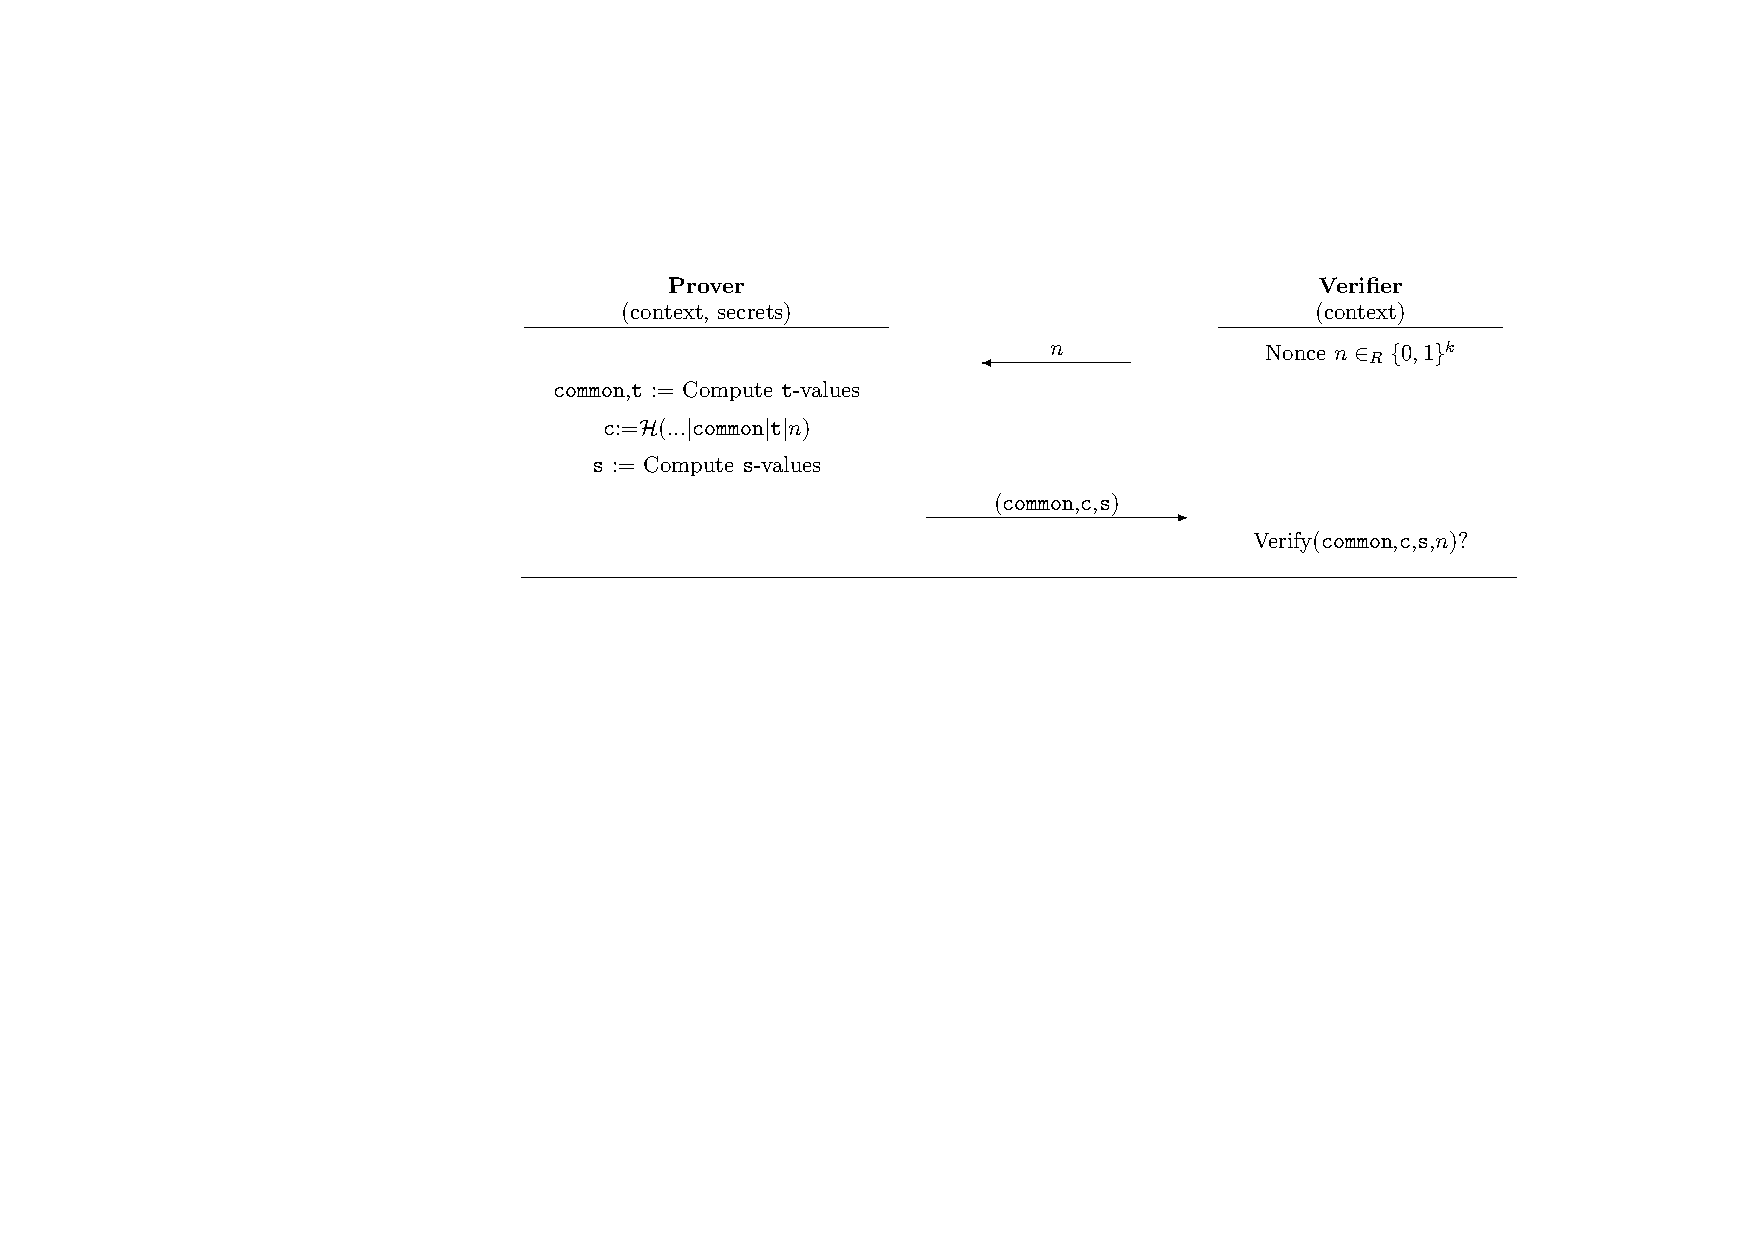
\includegraphics[width=\linewidth]{gfx/niZKPnonce}
	\caption{Identity Mixer's Non-Interactive ZKP with Nonce.}
	\label{fig:niZKPnonce}
\end{figure}

Fig. \ref{fig:niZKPnonce} shows the Idemix Proving scheme, where prover and verifier share a context information, the verifier generates the nonce, and the prover, non-interactively, computes the proof. The \texttt{common} values are equivalent to Schnorr's $t$, which was shared between prover and verifier. The verifier can recover some \texttt{\^t}-values from \texttt{common}, \texttt{c} and the \texttt{s}-values. This is equivalent to recovering Schnorr's $t$ from $g^{s_\alpha} y^c$. The verifier then checks whether or not \texttt{c} equals $\mathcal{H}$(...$\mid$\texttt{common}$\mid$\texttt{\^t}$\mid$$n$) to verify if the \texttt{\^t}-values are actually the \texttt{t}-values, making the proof valid.


Therefore, to describe any Idemix proof being performed by the User, one can focus on the key steps, compute the \texttt{t}-values, the challenge \texttt{c} and the \texttt{s}-values, and ignore the mathematical operations performed for each specific ZKP.



\subsection{System architecture}

The system will be compounded by the IoT device, the P2ABCE delegation server and the third party P2ABCE actors:

\begin{figure*}[htb!]
	\centering
	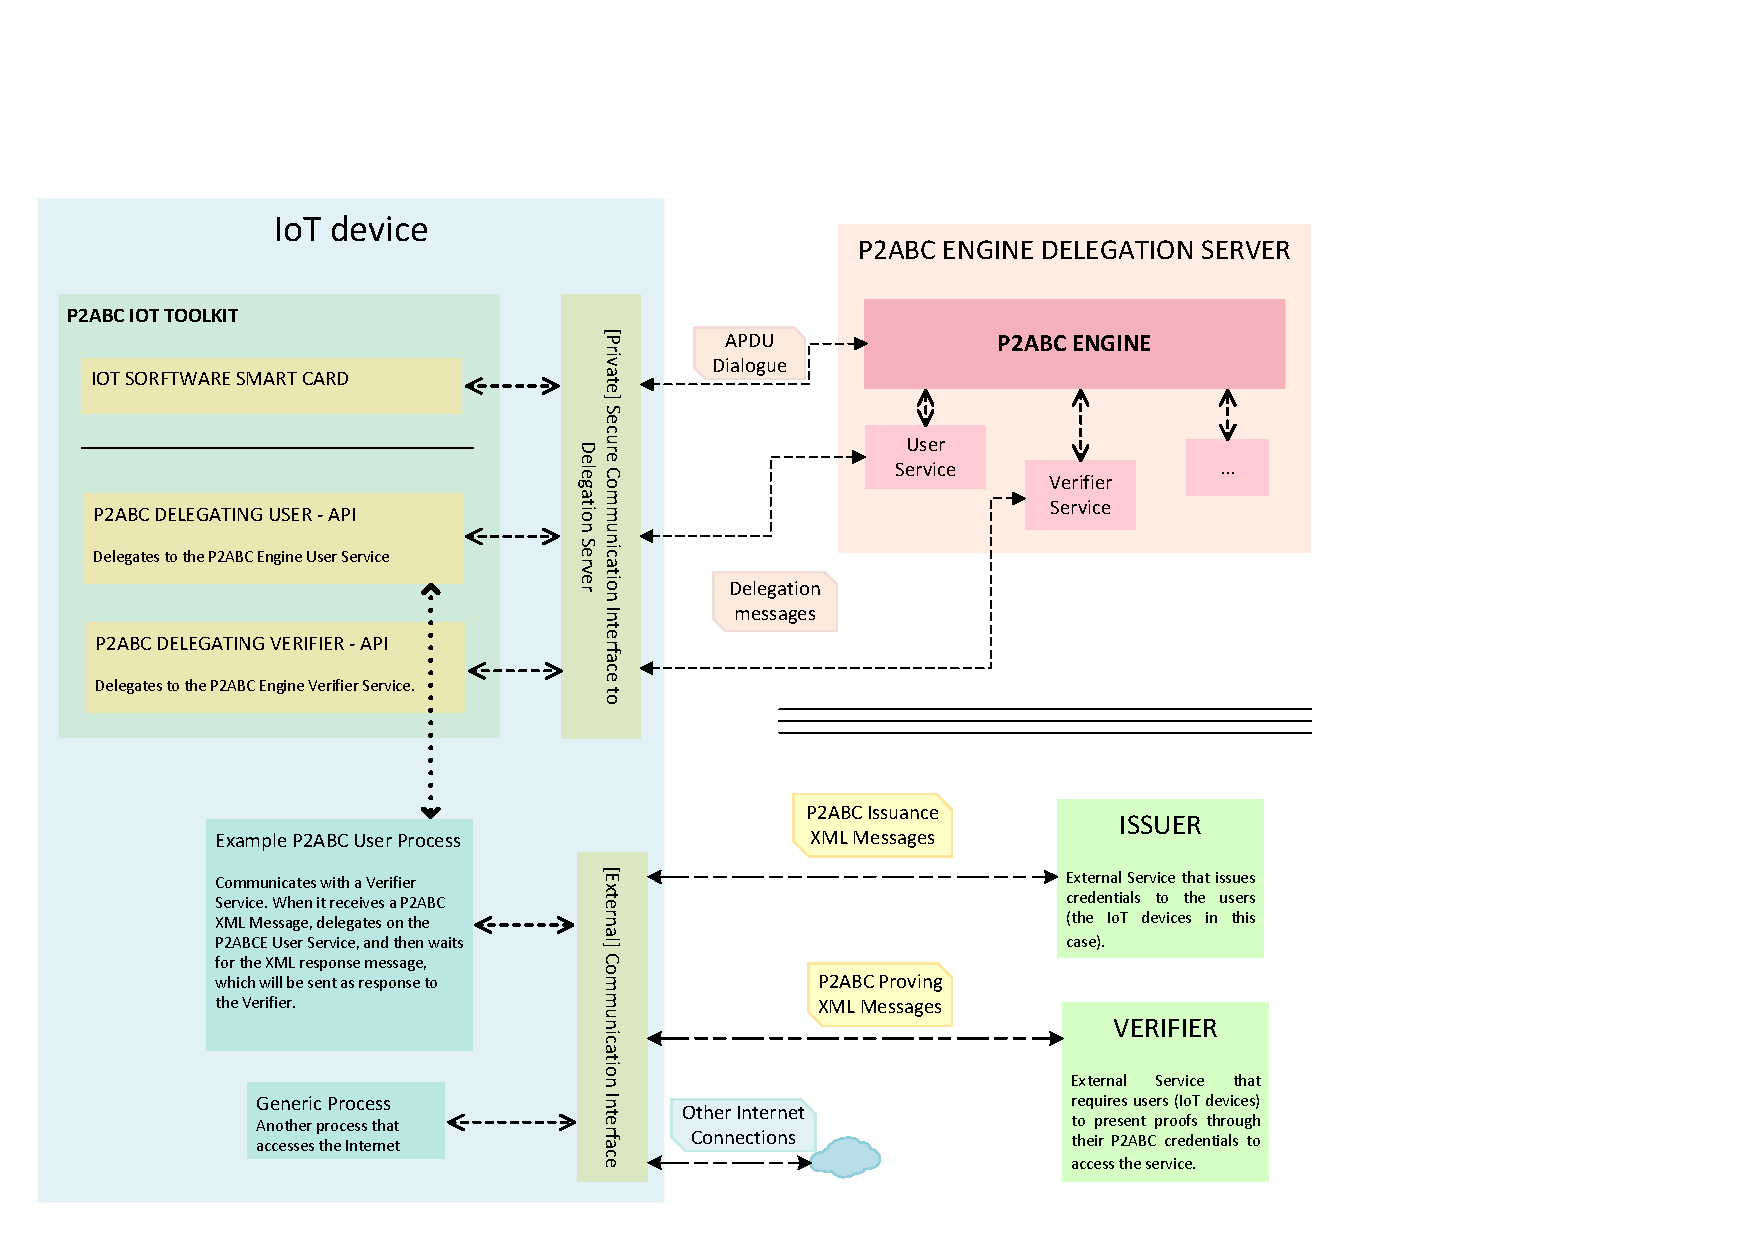
\includegraphics[width=0.7\textwidth]{gfx/P2ABCE-IoT-color}
	\caption{Proposed high level Architecture for integrating IoT devices in P2ABCE.}
	\label{fig:P2ABCE-IoT}
\end{figure*}



\begin{itemize}
	
	\item \textbf{IoT device}
	
	Figure \ref{fig:P2ABCE-IoT} shows our proposed architecture, in which the IoT device is represented with two communication interfaces. One allows external communications to other machines, including other P2ABCE actors. Through this interface, the P2ABCE XML messages are exchanged as in any traditional P2ABCE scenario. This lets an IoT device to interact with other actors without adaptations of the protocol. The other interface allows a secure communication channel with the delegation server. Both the delegation messages and the APDU Dialogue are transmitted over this interface, making it a point of attack that must be thoroughly secured.
	
	The scheme also shows the \textit{P2ABCE IoT Toolkit}. This piece of software includes the \textit{IoT Smart Card}, and the P2ABCE API.
	
	The \textit{IoT Smart Card} is the implementation of a software smart card, which listens for APDU Commands from the secure interface and stores securely the credentials and private keys within the device's memory.
	
	The P2ABCE API is an interface for other processes that wish to use the private-preserving environment of P2ABCE. It provides access to every operation available, hiding the delegation process to the server. In the future, for example, the Verification Service could be implemented to run entirely in the IoT device, then the toolkit would conceal the transition from delegation to native execution.
	
	
	\item \textbf{P2ABCE actors}
	
	The possible roles in a P2ABC system are the Issuer, the User, the Verifier, the Revocation Authority and the Inspector, where these last two actors are optional. All of them use the P2ABCE language to communicate to each other. Any third party actor that communicates with the IoT device will be unaware of the fact that the device is a constrained device, because it will accept and generate the same XML as a traditional User.
	
	Figure \ref{fig:actors} showcases the different actors and their interactions, where the User is in the center, which receives a credential from an Issuer, can generate privacy-preserving Tokens for Verifiers or revoke an stolen credential. The Inspector is the only entity capable of reading some ciphered attributes from a Token, if the User accepted to include that ciphered information in it. It serves the Law Enforcement authorities, warrant granted, to track any misuse of a credential.
	
	
	\item \textbf{P2ABCE Delegation Server}
	
	The machine in charge of receiving commands from authorized IoT devices to parse the XML files exchanged. It will also orchestrate through APDU Commands the cryptographic operations the IoT smart card must perform.
	
	
\end{itemize}

\begin{figure}[bth]
	\centering
	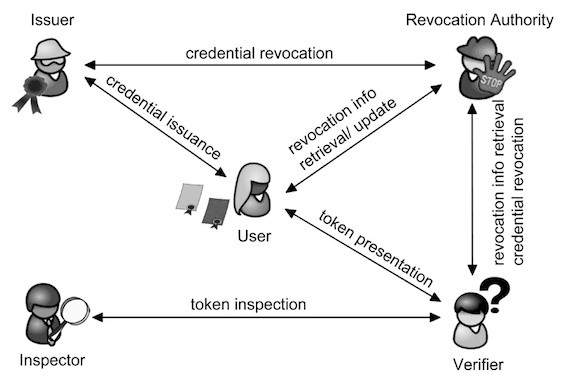
\includegraphics[width=0.8\linewidth]{gfx/actors.jpg}
	\caption{Entities in a P2ABC System. Source: P2ABCE project.}
	\label{fig:actors}
\end{figure}


\subsection{Delegation process}

This section describes the computation offloading carried out by the IoT device. The steps the device will perform in any kind of interaction are:

\begin{itemize}
	\item Communication with P2ABCE actor
	
	The IoT device, acting as a User, starts an interaction with another actor. If it is an Issuer, it will start the issuance process. If it is a Verifier, then it will provide a Presentation Policy for the device to proof in a privacy preserving way. Figure~\ref{fig:DelegationProving} shows an example of this last case.
	
	It may also happen that the device is contacted as a Verifier by another actor, e.g. in a M2M scenario where the IoT device requires authentication to access to its resources.
	
	\item Delegation to the P2ABCE Server
	
	Depending on what role the IoT device is acting as, it will use the corresponding API from the P2ABCE IoT Toolkit. The selected API will delegate to the Service deployed in the delegation server, e.g. User Service. The delegation message will include the XML data, and any parameter required to accomplish the task, as the information on how to communicate back with the IoT smart card.
	
	The server will then parse the XML messages and begin to orchestrate the response. In the case of the Verifier Service, it will answer immediately with an \textit{accept} or \textit{reject} of the Token. In case it is the User Service, it will need information from the IoT credentials and cryptographic operations.
	
	\item APDU Dialogue
	
	Through the secure channel between IoT device and server, the User Service will send APDU Commands to the  \textit{IoT smart card} to read the credential information or perform cryptographic operations involving private keys, necessarily stored inside the IoT device.
	
	During a proof, the Service will read the credential public information to fill the Presentation Token, and then will request the IoT smart card to calculate the \texttt{t}-values of the proof. The Service will read the \texttt{common} and \texttt{t}-values, use the nonce present in the Presentation Policy of the Verifier and compute the challenge \texttt{c}. Next, the Service will send \texttt{c} to the IoT smart card through another APDU Command to request the calculation of the \texttt{s}-values.
	
	After the APDU Dialogue, the Service has all the needed values to fill in the Token, and the IoT device performed all the operations involving private values on its own.
	
	
	\item Server response
	
	After the APDU Dialogue, if needed, the server may return a status code indicating success or failure, or a XML response if the third party actor requires an answer from the IoT device, as a Presentation Token, or the intermediate issuance messages.
	
\end{itemize}

\begin{figure}[bth]
	\begin{center}
		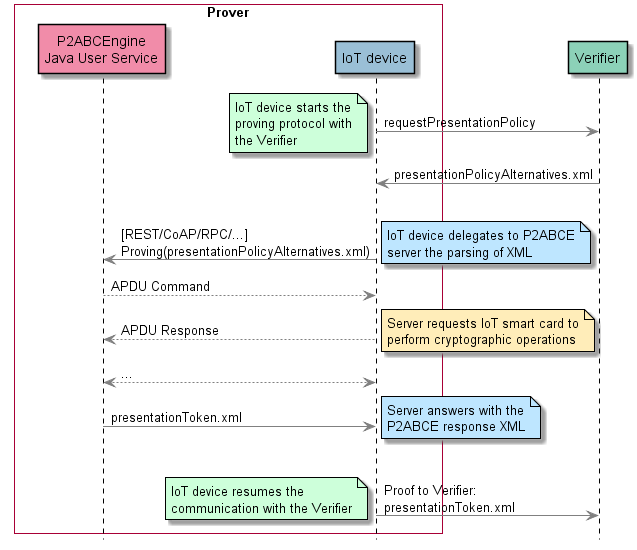
\includegraphics[width=\linewidth]{gfx/UML/provingDelegation}
	\end{center}
	\caption{Messages exchanged during the proving delegation.}
	\label{fig:DelegationProving}
\end{figure}



The \textit{Server-IoT} channel must be secured. It must avoid impersonation of the P2ABCE delegation server or authorized devices. For this purpose many traditional solutions already exist. The delegation server could be in a local network, or physically attached to the IoT device, like the Arduino Y\'un\footnote{\url{https://www.arduino.cc/en/Main/ArduinoBoardYun}} combines an ATmega and an Atheros with Linux. The choice may depend on the particular deployment.

%Transmissions over the \textit{Server-IoT} channel must be secured in order to avoid attacks like impersonating the P2ABCE delegation server, an attacker sending APDU Commands to the IoT smart card, or delegating as a device to the server but giving the parameters of another device, making the delegation server send the APDU Commands to a victim IoT smart card.


%We could use a corporative PKI to issue certificates to the server and devices and configure policies for access control; design a challenge-response system combined with the smart card PIN, like a password and TOTP\footnote{Time-based One-time Password} in a 2FA\footnote{Two-factor authentication} login. We also could connect physically the delegation service through RS-232 serial to the IoT device, securing both physically as        we      would do with the IoT device on its own, isolating the delegation system from any network attack. % This last idea is an approximation to the Arduino Y\'un\footnote{\url{https://www.arduino.cc/en/Main/ArduinoBoardYun}}, a development board that integrates two microcontrollers, one a typical Arduino with very low resources, and another one running a fork of OpenWrt. The Arduino microcontroller can control the terminal of the more powerful one, using the serial pins as commented before.

%As      we        can see, there are many state of the art solutions for all this threads, therefore,           we       can assume a secure channel without mentioning a specific solution, providing freedom to choose the most fitting one in a real deployment.

%%%%%%%%%%%%%

%Regarding the definition of the P2ABCE API, it is a work in progress, and in the meantime,         we           will work with the REST API currently available in the P2ABCE project to perform the delegation. Regarding the \textit{IoT Smart Card}, the P2ABCE project defines the APDU instructions with the corresponding format of the APDU Commands and Responses. In the next section we will explain the PoC for IoT based on these P2ABCE specifications.



%%%%%%%%%%%%%




\section{Proof of Concept Implementation}\label{ch:implementation}
% +Implementation:
% *System:
% 	-Raspbian OS: distro de debian para Raspberry Pi, que se describirá en los tests
% 	-LEDE: ash terminal (shell command interpreter), POSIX, typical hardware, libraries with no hardware aceleration vs smart card MULTOS,
%
% *Delegation
%  -REST as current delegation protocol: curl script bash
%  -BIOSC as current APDU transmission protocol: no security -> no overload.
% *Smart Card
%  
%  -IoT Smart Card software design and implementation notes.
%  -Sequence diagrams. TODO


In this section we present the first PoC implementation, introducing the IoT system where we are going to work, then we will describe the delegation protocols, one for the computation offloading of the IoT device on the P2ABCE server, and another for the transmission of APDU Commands, and finally, we will describe the IoT smart card implementation.

We will develop our PoC in Linux based systems aimed for IoT environments, that will serve as a starting point for future implementations in more constrained devices or different systems.

In our delegation server we will run Raspbian OS in a Raspberry Pi3, and for our IoT device, we will use LEDE, Linux Embedded Development Environment, a distribution forked from OpenWrt, aimed for routers and embedded chips with low resources requirements.



\subsection{PoC Delegation}

The delegation process has two steps, first the IoT device calls the P2ABCE server to offload the parsing of the XML data, and then the P2ABCE server sending APDU Commands to the IoT smart card in the device.


\subsubsection{PoC Delegation to the P2ABCE Server}


Currently P2ABCE offers multiple REST web services to run different roles in P2ABCE system: User Service, Issuer Service, Verification Service, etc. 
%Any third party application that integrates P2ABCE with their system can make use of these services or implement the functionality using the library written in Java, the tool that the REST services actually use.
%
%In this PoC, the P2ABCE's User Service needed to be modified, because this is the role the IoT device plays. We added the following REST call:
%\begin{center}
%	\textit{/initIoTsmartcard/{issuerParametersUid}?host=\&port=}
%\end{center}
%where we communicate the P2ABCE server that an IoT Smart Card is accessible via the IP address \textit{host} and TCP port \textit{port}.
After an analysis of P2ABCE's code, the \texttt{HardwareSmartcard} class implements the \texttt{Smartcard} interface using the package of abstract classes \texttt{javax.smartcardio} to communicate with the physical smart cards. The Oracle JRE implements these package for the majority of smart card manufacturers. For our PoC, we implement the \texttt{javax.smartcardio} package so it transmits the APDUs with our custom protocol, making the use of a physical or IoT smart card totally transparent to the \texttt{HardwareSmartcard} class, enhancing maintainability, and following the \textit{expert pattern} from the known GRASP guidelines.

In this PoC, the P2ABCE's User Service was modified to add a new method receiving the IoT device's  IP address and a port where the IoT Smart Card will be listening for the APDU Commands.
This method creates a new \textit{HardwareSmartcard} object, but instead of the \textit{javax.smartcardio} Oracle's \textit{CardTerminal} implementation, we use our own \textit{IoTsmartcardio} implementation for the \textit{HardwareSmartcard} constructor.


The remaining REST methods are left untouched, and will serve to parse the XML files exchanged.

\hfil

\subsubsection{APDU Dialogue Transmission}


To transmit the APDU messages in our PoC we use a simple protocol, that we will refer as BIOSC (Basic Input Output Smart Card). It consists on one byte for the instruction, that can mean either an APDU Commnad or a finishing instruction to close the connection.

In the first case, the header continuous with two more bytes for the length of the payload bytes to read, which are the APDU Command bytes.
To send an APDU Response in BIOSC, the IoT device sends back to the server two bytes for the length and then the raw APDU Response bytes. The messages are sent over TCP for a reliable transmission.

We lack any security (authentication or authorization) that a real system should implement. It is vital to authenticate the delegation service, to authorize it to perform APDU Commands, and the same with the IoT device, to prevent impersonation attacks. But using BIOSC for the transmission of the APDU messages in the PoC, with only 3 bytes of overhead, helps us in the  benchmarks to measure the real performance of the system.


\subsection{IoT Smart Card Implementation}

In this section we present the code architecture and sequence diagram of the IoT Smart Card PoC, based on ABC4Trust's Card Lite.

\hfil

\textsc{Code structure}
We divide the project in three different sections with the objective of enhancing maintainability, improving future changes, ports, fixes, etc.
In \autoref{fig:IoTCScomponents-bw} we show how the project is structured in three sections:

%\begin{figure}[bth]
%	\begin{center}
%		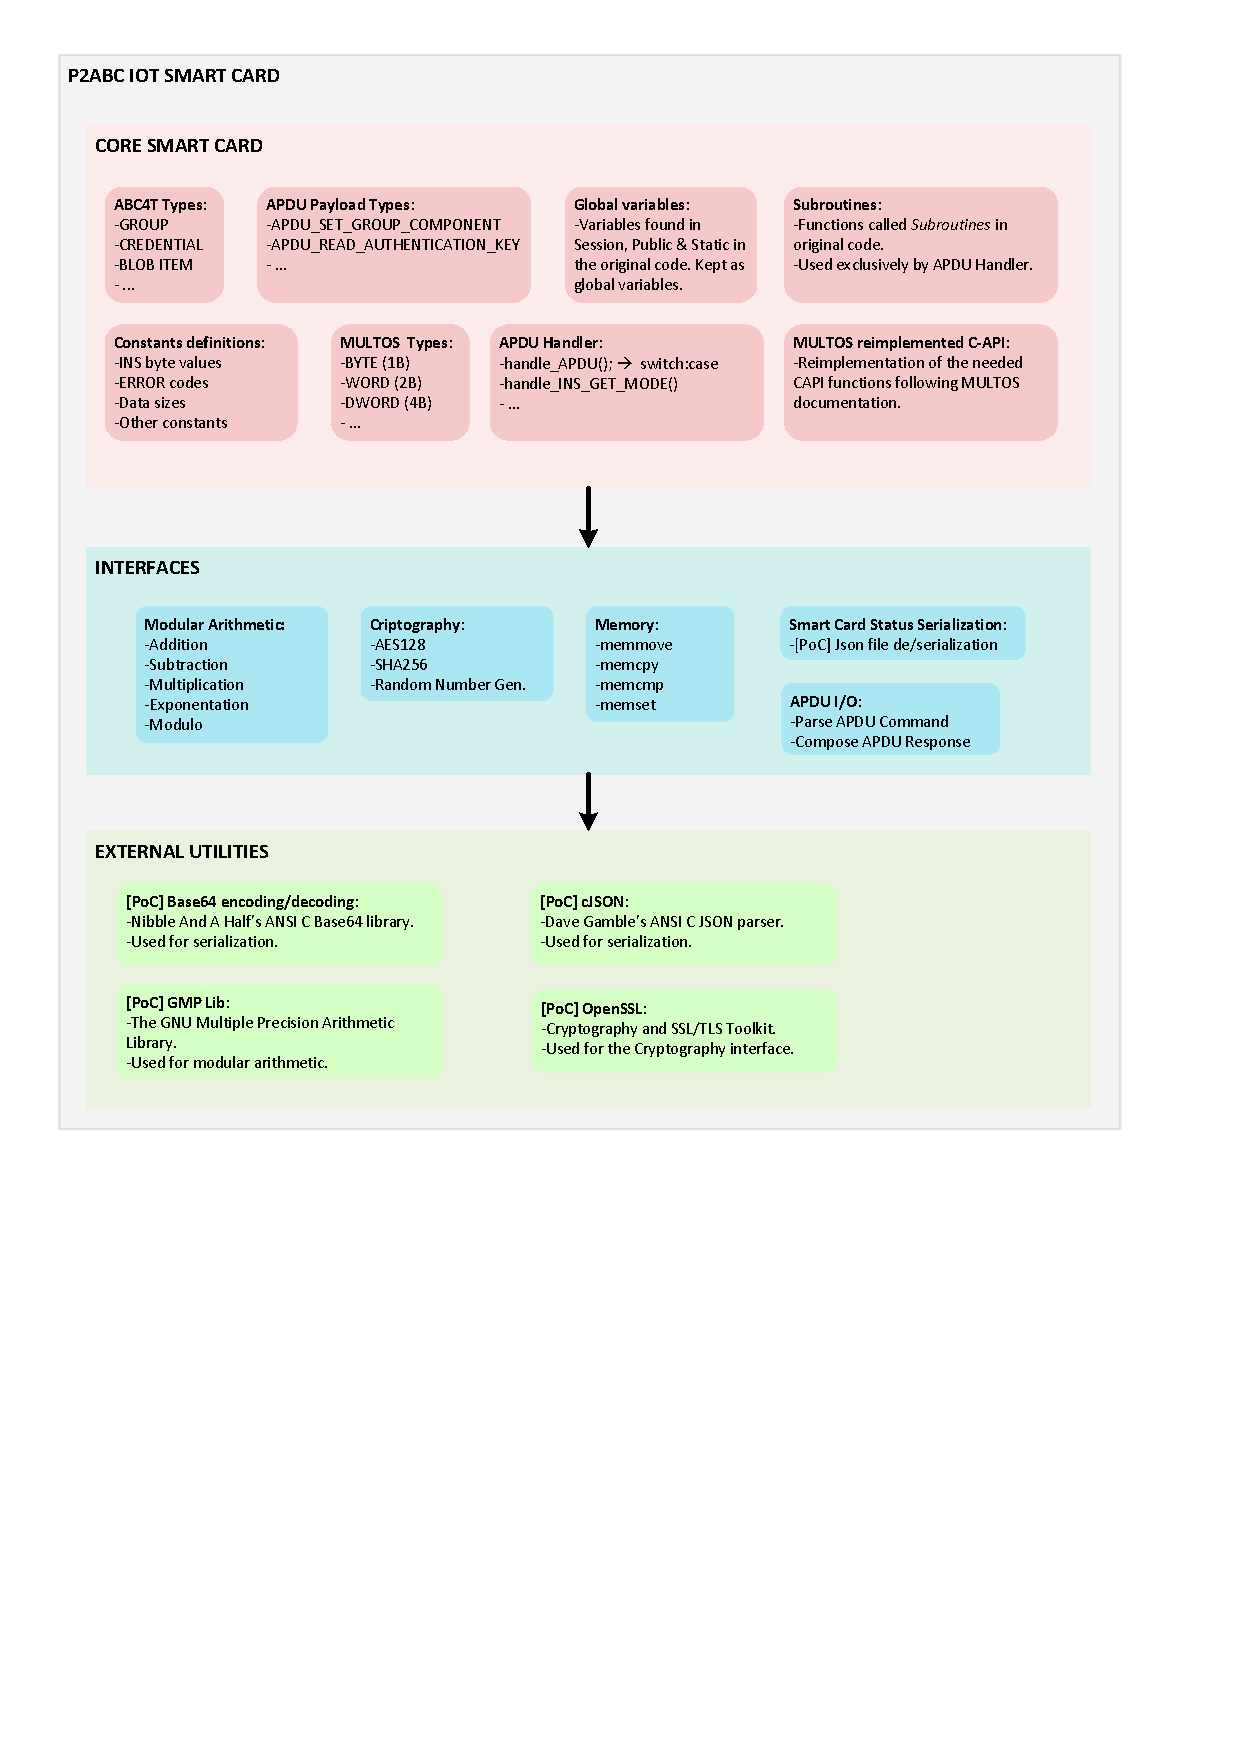
\includegraphics[width=\linewidth]{gfx/IoTCScomponents-color}
%	\end{center}
%	\caption{IoT Smart Card Code Structure.}
%	\label{fig:IoTCScomponents-color}
%\end{figure}

\begin{figure}[bth]
	\begin{center}
		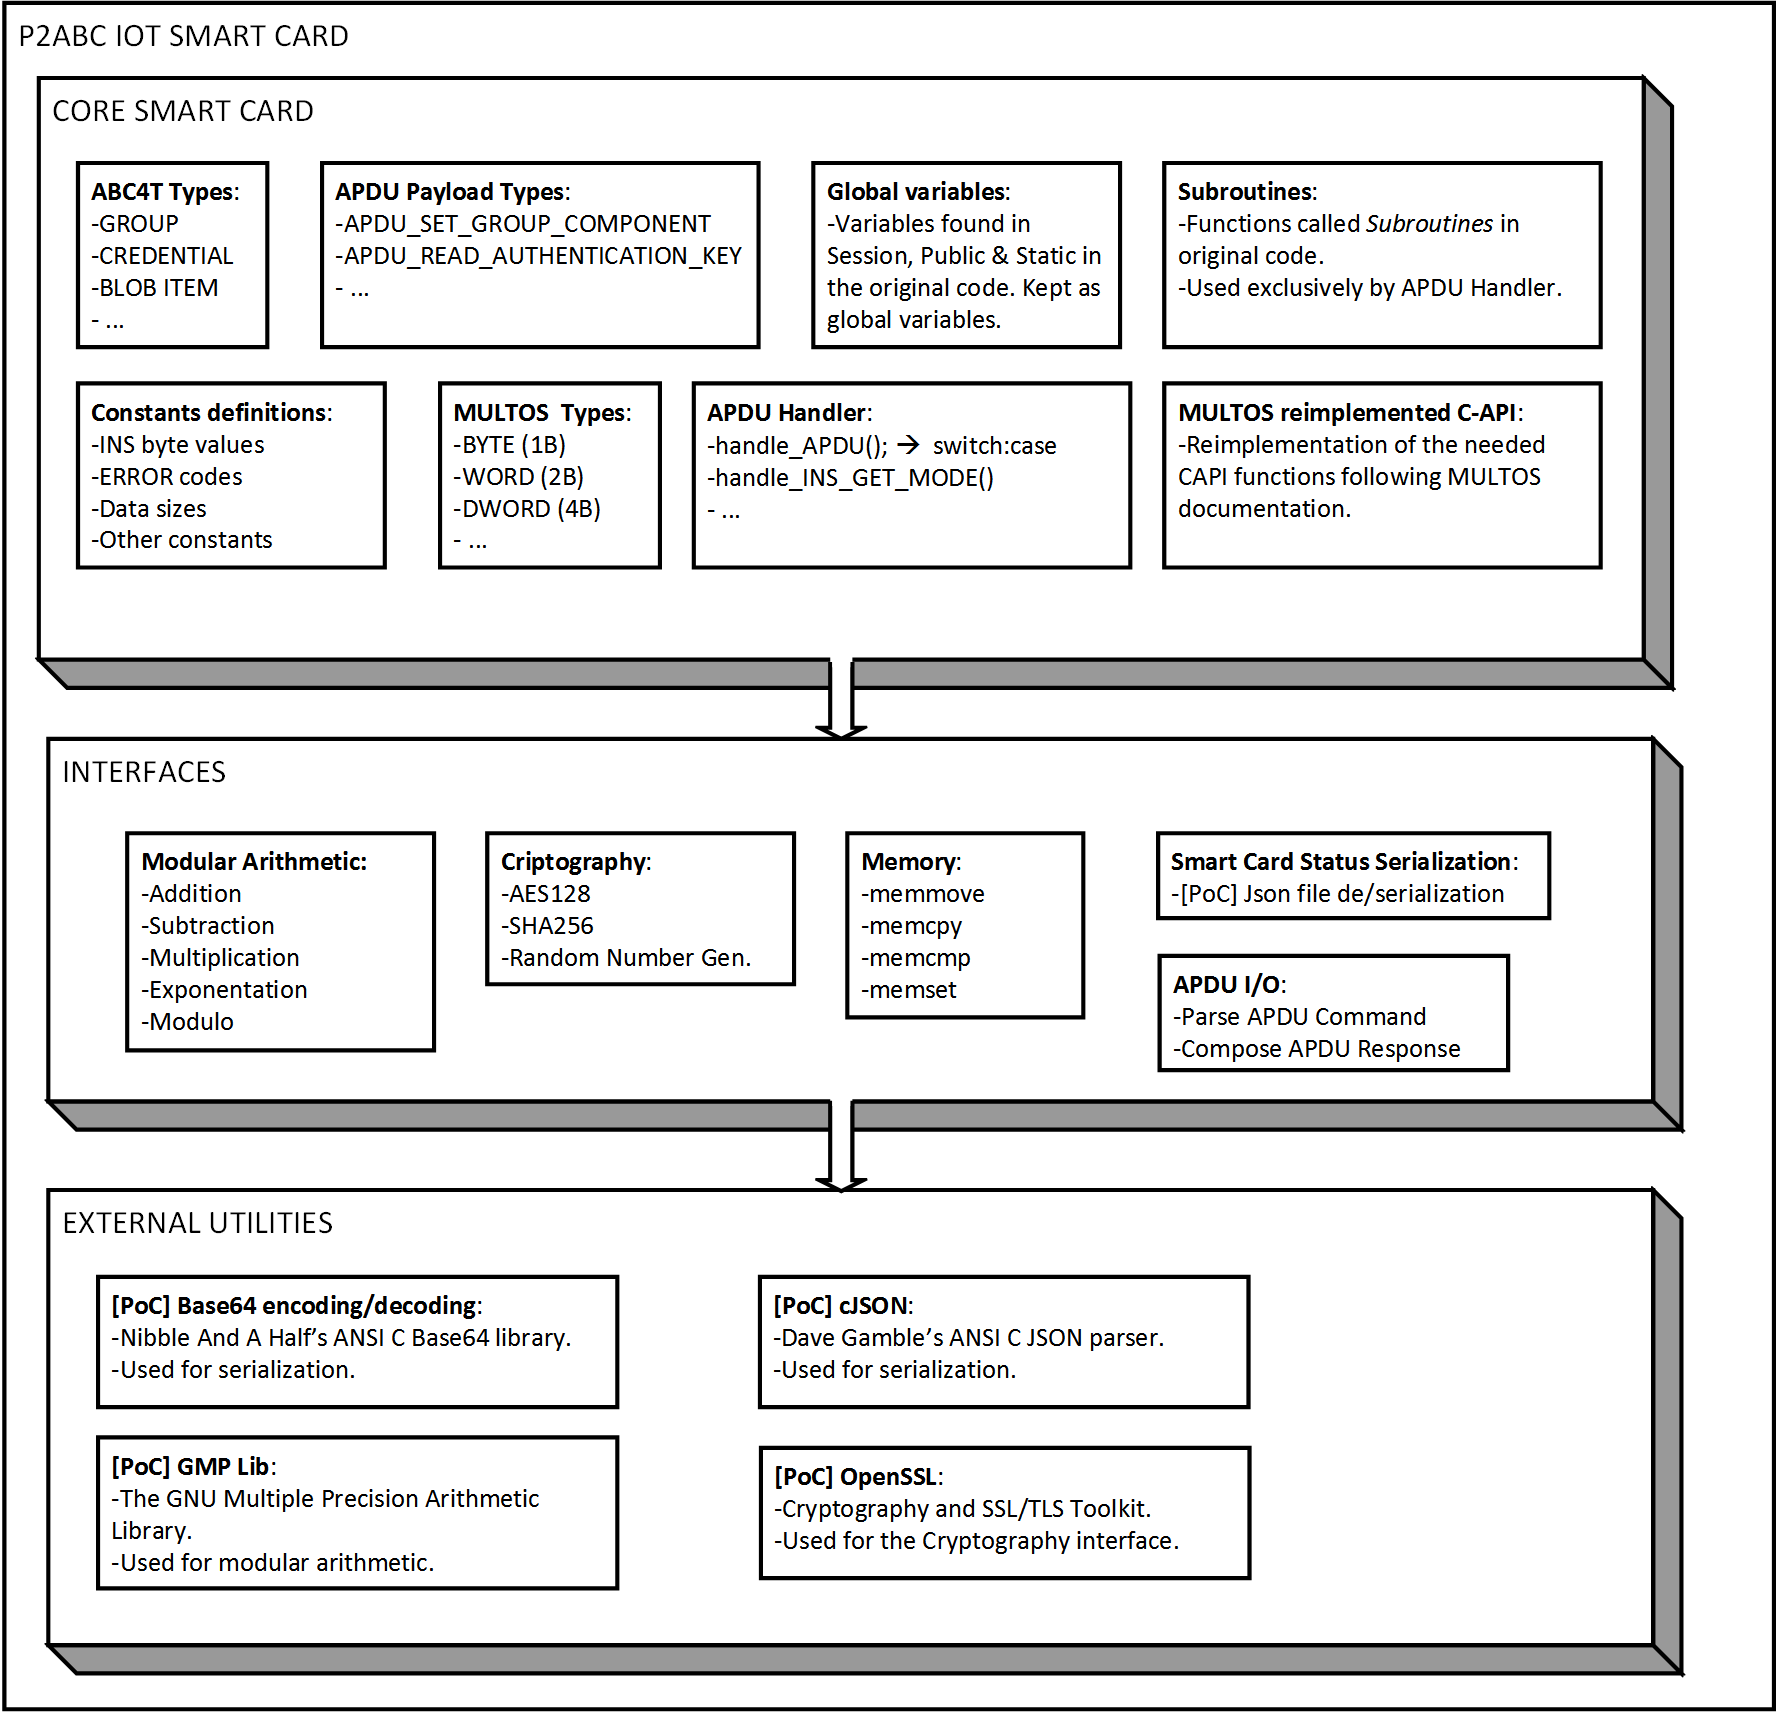
\includegraphics[width=\linewidth]{gfx/IoTCScomponents-bw}
	\end{center}
	\caption{IoT Smart Card Code Structure.}
	\label{fig:IoTCScomponents-bw}
\end{figure}


\hfil

\textbf{Core smart card:} The smart card logic lies here, with the concepts of APDU Commands, the instructions that are defined for P2ABCE smart cards, and how to process them and generate proper APDU Responses.

Here we adapted the ABC4Trust Card Lite's code. However, the ABC4Trust's code heavily depends on the MULTOS platform, therefore, we reimplement the used MULTOS functions following the documentation, adapting it in some cases for \textit{expanded functionality}, to avoid some MULTOS API limitations, like in \cite{vullers2013efficient}, when they noted that MULTOS' \texttt{ModularExponentiation}  function does not accept exponents larger than the modulus size, so they implemented \texttt{SpecialModularExponentiation}.

MULTOS compiler does not apply data structure alignment. This affects the inherited ABC4Trust's code because of the use of \texttt{memcpy} to copy multiple variables in one call.%, for example, the APDU Command payload usually includes multiple data, and instead of copying one variable at a time, the \texttt{struct} is defined with the same order and copies everything at once.

The temporal solution is to use \texttt{struct \_\_attribute\_\_((\_\_packed\_\_))} to ask a GCC compiler to not use padding in the structs, but this is not standard, neither a good practice. A deeper refactorization of the code is needed where the hidden copies of variables must be made explicit, letting the compiler manage the memory layout on its own.

\hfil

\textbf{Interfaces:} To reimplement some of the MULTOS functions, we defined a facade to isolate the implementation of the core smart card from our different options, that could vary depending on the hardware or the system used by the IoT device.
With this facade we could, for example, change the implementation of cryptographic functions with a hardware implementation (e.g. Atmel's chips for SHA and AES), or software implementations optimised for the target platform.

The interfaces defined can be organized in 5 groups (see \autoref{fig:IoTCScomponents-bw}), depending on their purpose: Modular Arithmetic, Cryptography, Memory Management, Serialization and APDU Parsing.

\hfil

\textbf{External utilities:} In our PoC we used two ANSI C libraries, for base64 and JSON, and two shared libraries available as packages in LEDE: GMPLib and OpenSSL. These libraries use dynamic memory and offer more functionality than we need, and although they are useful tools for the early development versions of the PoC, future versions should use more lightweight solutions.

\hfil

The \textit{interfaces} and \textit{external utilities} sections  allow that the project is easily ported to specific targets without modifying the smart card logic.


\hfil

\textsc{Execution workflow}

The sequence diagram from \autoref{fig:sequenceBIOSC} shows the execution of the PoC IoT smart card.



\begin{figure}[bth]
	\begin{center}
		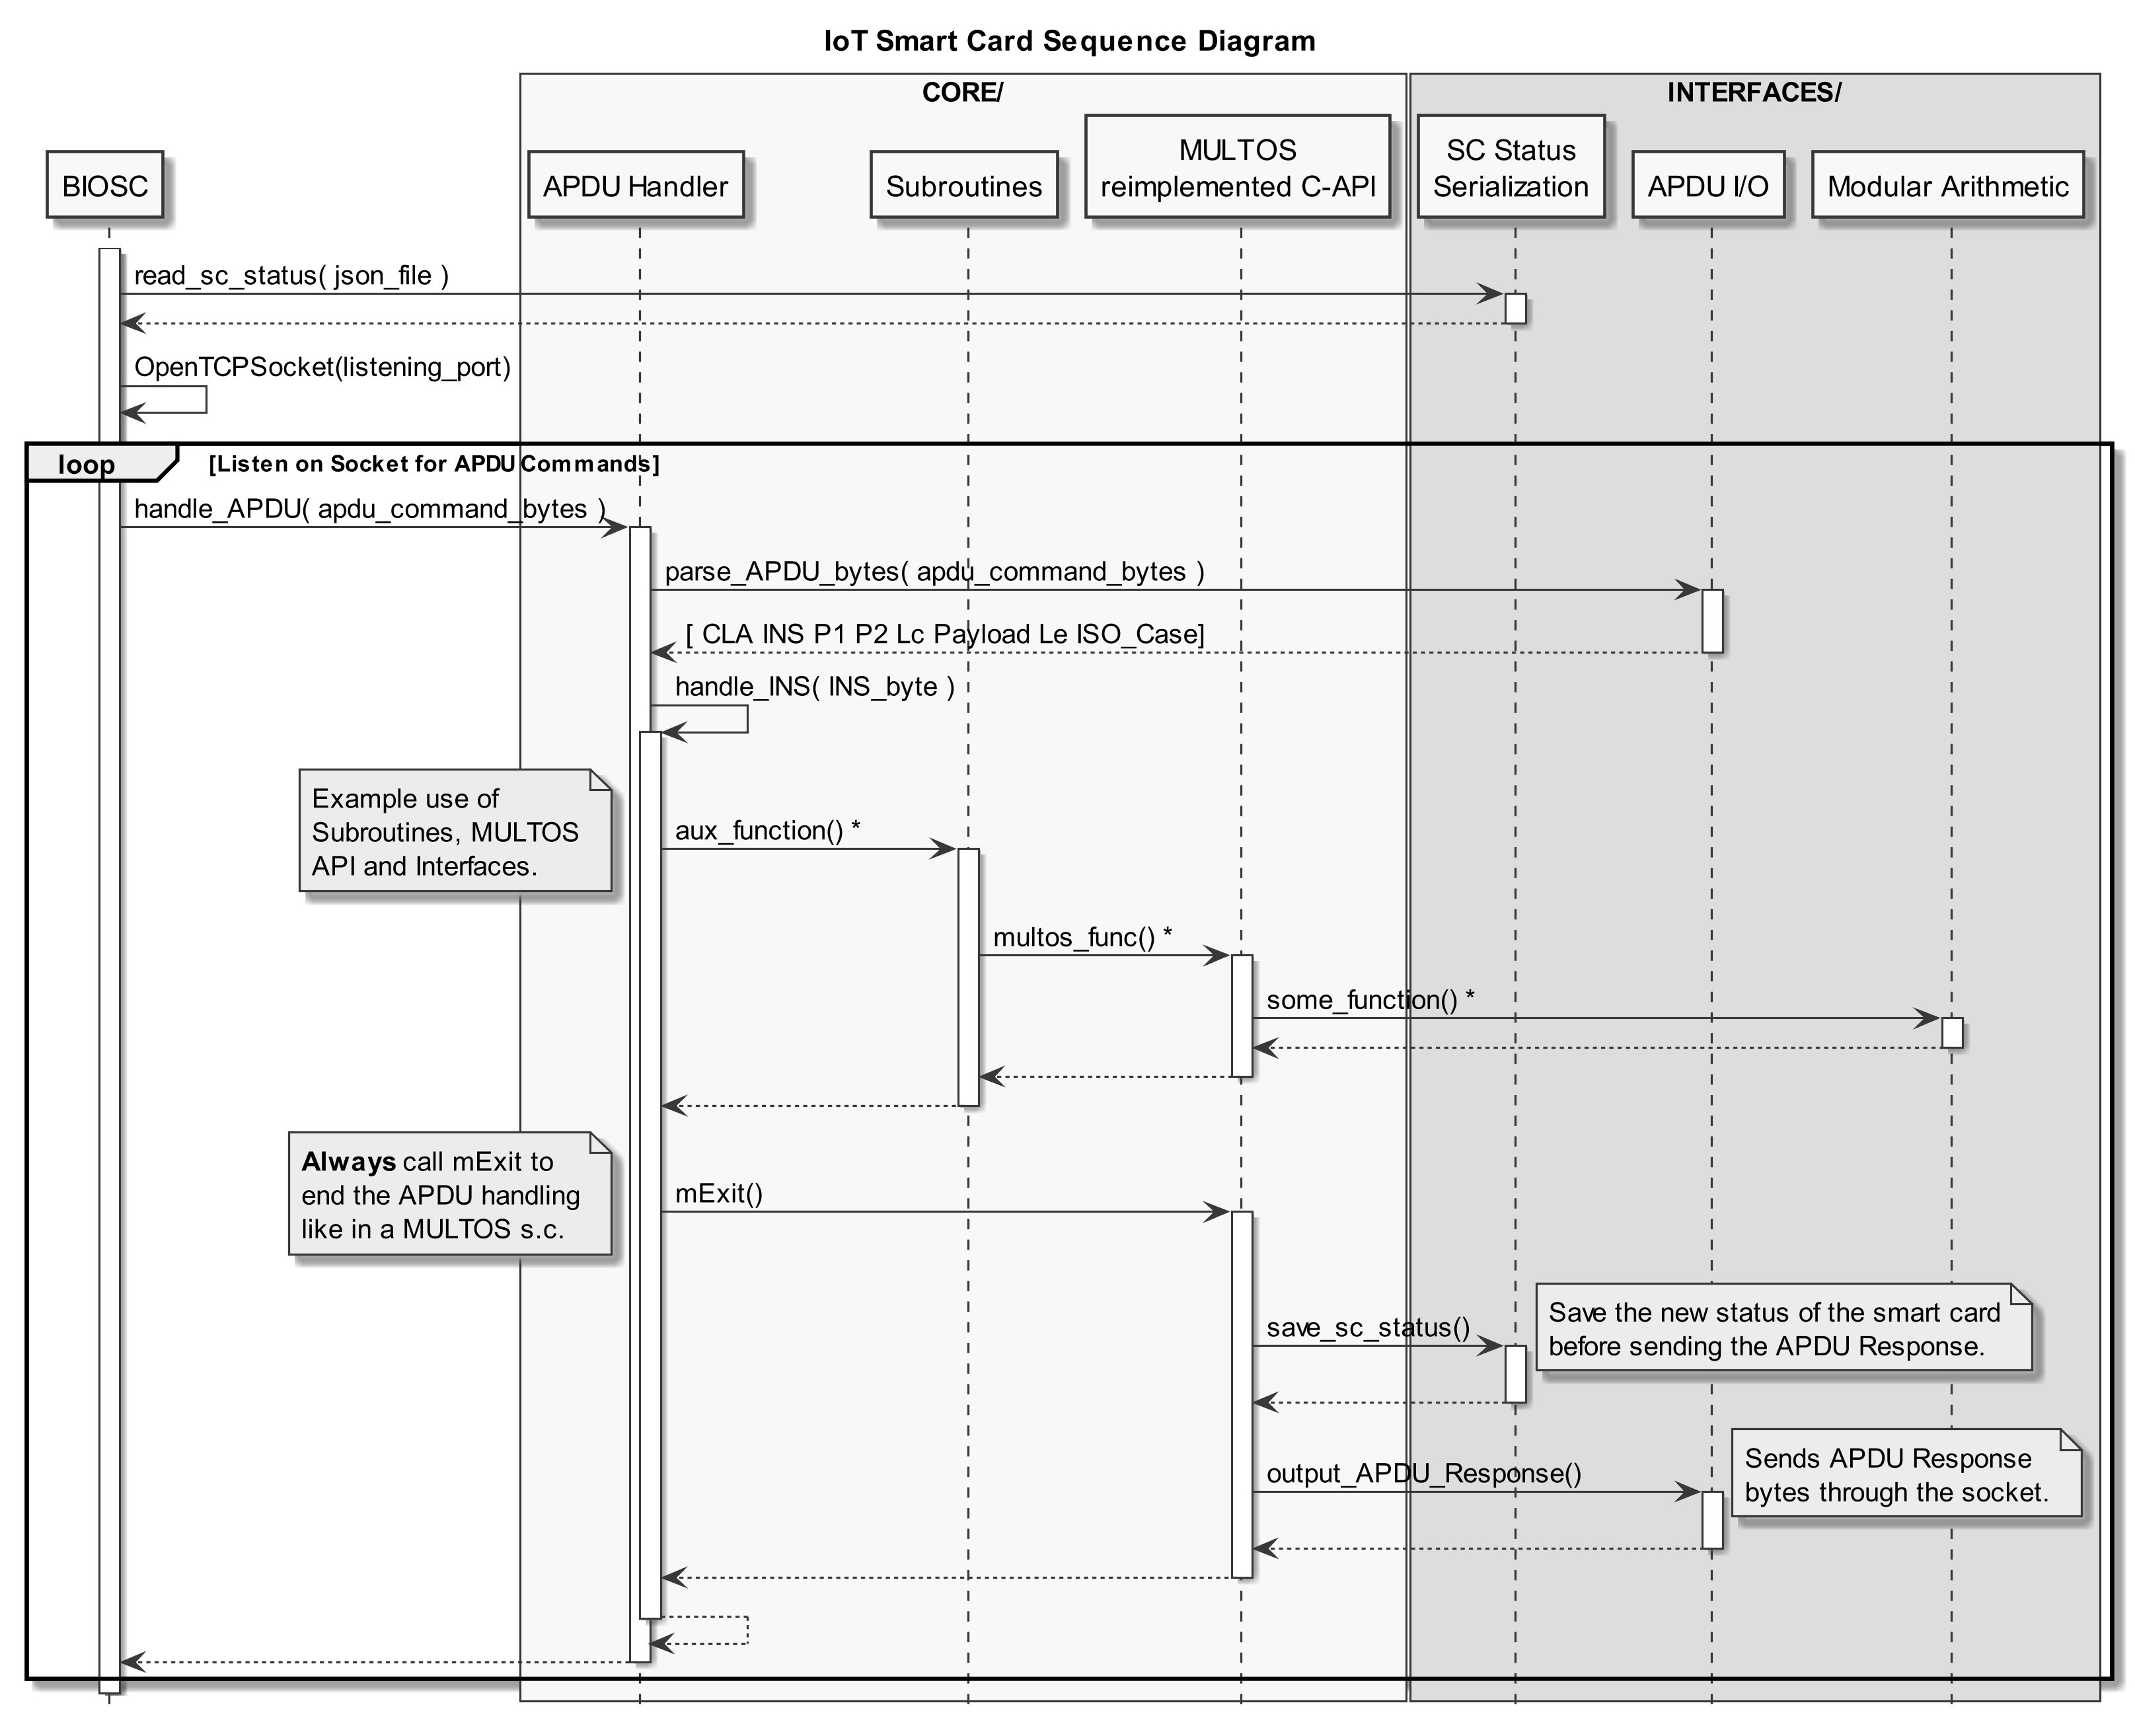
\includegraphics[width=\linewidth]{gfx/UML/sequenceBIOSC}
	\end{center}
	\caption{IoT Smart Card Sequence Diagram.}
	\label{fig:sequenceBIOSC}
\end{figure}



The program starts with the \texttt{main} function in BIOSC, that deserializes the status from the Json file, and listens on a loop for APDU Commands from the delegation server.

Every time an APDU Command arrives, it calls the function \texttt{handle\_APDU()} with the raw APDU bytes. The Handler calls the APDU I/O interface to parse the bytes, storing in global variables the APDU structure. Using a \texttt{switch-case} expression on the \texttt{INS} byte, the Handler calls an \textit{Instruction handler} function.

Inside this function, it may call multiple functions from the Subroutines, that may call MULTOS C-API functions, which, in turn, may use an interface to perform its functionality.

Finally, every instruction handler must end, before the \texttt{return;} expression, with a call to \texttt{mExit}. This reimplemented MULTOS function will save the current status of the smart card and send the APDU Response back to the delegation server.

After returning from these functions, \texttt{mExit}, the instruction handler and the APDU handler, the program listens again from the socket.





%************************************************
\section{Validation and Performance Evaluation}\label{ch:validation}
%************************************************

% TODO:
% https://abc4trust.eu/download/D4.2%20Final%20Reference%20Implementation.pdf
% Comparar con página 44

This section describes the deployment of three testing scenarios: a laptop, a standalone Raspberry Pi 3, and an Omega2 IoT device with the Raspberry Pi 3 as the delegation server. We will measure and compare the results to determine if the proposed solution runs as expected and is feasible.

\subsection{Testbed description}

%First, we shall describe the example Attribute Based Credential system in use. Then, the hardware we will use in our benchmarking.

%\subsubsection{P2ABCE setting}

To verify the correct execution of the \textit{IoT smart card}, the test is based on the ABC system from the tutorial in the P2ABCE Wiki\footnote{\url{https://github.com/p2abcengine/p2abcengine/wiki/}}. It consists on a soccer club, which wishes to issue VIP-tickets for a match. The VIP-member number in the ticket is inspectable for a lottery, ie. after the game, a random presentation token is inspected and the winning member is notified.

First, the \textbf{setup} phase takes place, where several artifacts are generated and distributed to the various P2ABCE entities. Next, a ticket credential containing the following attributes is \textbf{issued}:
\begin{Verbatim}[fontsize=\footnotesize]
First name: John	Member number: 23784638726	
Last name: Dow	  Matchday: 2013-08-07Z
Birthday: 1985-05-05Z
\end{Verbatim}

%During the \textbf{issuance}, a \textit{scope exclusive pseudonym} is established and the newly issued credential is bound to this pseudonym. This ensures that the ticket credential can not be used without the smart card.

Then \textbf{presentation} is performed, where a \textit{presentation policy} from the verifier specifies that the member number is inspectable and a predicate ensures that the matchday is in fact $2013-08-07Z$. This last part ensures that a ticket issued for another match can not be used.

\hfil

%\subsubsection{Execution environment}

First we will execute the test in our development machine (laptop). After asserting that the services work as expected, we then run the test in a Raspberry Pi 3\footnote{\url{https://www.raspberrypi.org/products/raspberry-pi-3-model-b/}}, exactly like in the laptop. Finally, we will deploy the IoT smart card in an Omega2\footnote{\url{https://docs.onion.io/omega2-docs/omega2.html}} and the delegation services in the Raspberry Pi 3. After every test, we checked that the issuing and proving were successful, in case a cryptographic error appeared in the implementation.
A downside of using the Omega2 is the lack of hardware acceleration for cryptographic operations, unlike the MULTOS smart cards.



\paragraph{The network} In our third scenario, the Raspberry Pi 3 and the Omega2 will talk to each other over TCP. This implies possible network delays depending on the quality of the connection. The Raspberry Pi 3 is connected over Ethernet to a switch with WiFi access point. The Omega2 is connected over WiFi n to said AP. To ensure the delay wasn't significant, we measured 6000 APDU messages taken from previous executions, and the results show that the mean transmission time is less than half a millisecond per APDU. From our analysis of the tests we conclude that the network time is negligible compared to the rest of the computations.



\subsection{Results}

After 20 executions for each scenario (laptop, RPi3, Omega2+RPi3), we measure the time of each REST call executed against the User Service in the delegation server and take the means to compare each step of the testbed. Because during a call to the User Service, the server may contact the \textit{IoT Smart Card}, the difference in times between the second and third scenario will show the performance of our IoT PoC.

It is worth noting that during the tests, the CPU usage showed that P2ABCE does not benefit from parallelization, therefore it only uses one of the four available cores in the laptop and Raspberry Pi 3.

%\paragraph{The setup}\hfil
\hfil

The IoT device does not intervene in the first step of our testbed, the setup, until the initialization of the new smart card, thus the times measured for each REST call in the second and third scenarios are practically identical as we can see in Fig.~\ref{fig:setup:graph}. the laptop is about ten times faster than Raspberry Pi 3. It is also noticeable that the setup step is only done once, and the highest time measured is less than two and a half seconds.

\begin{figure}[bth]
	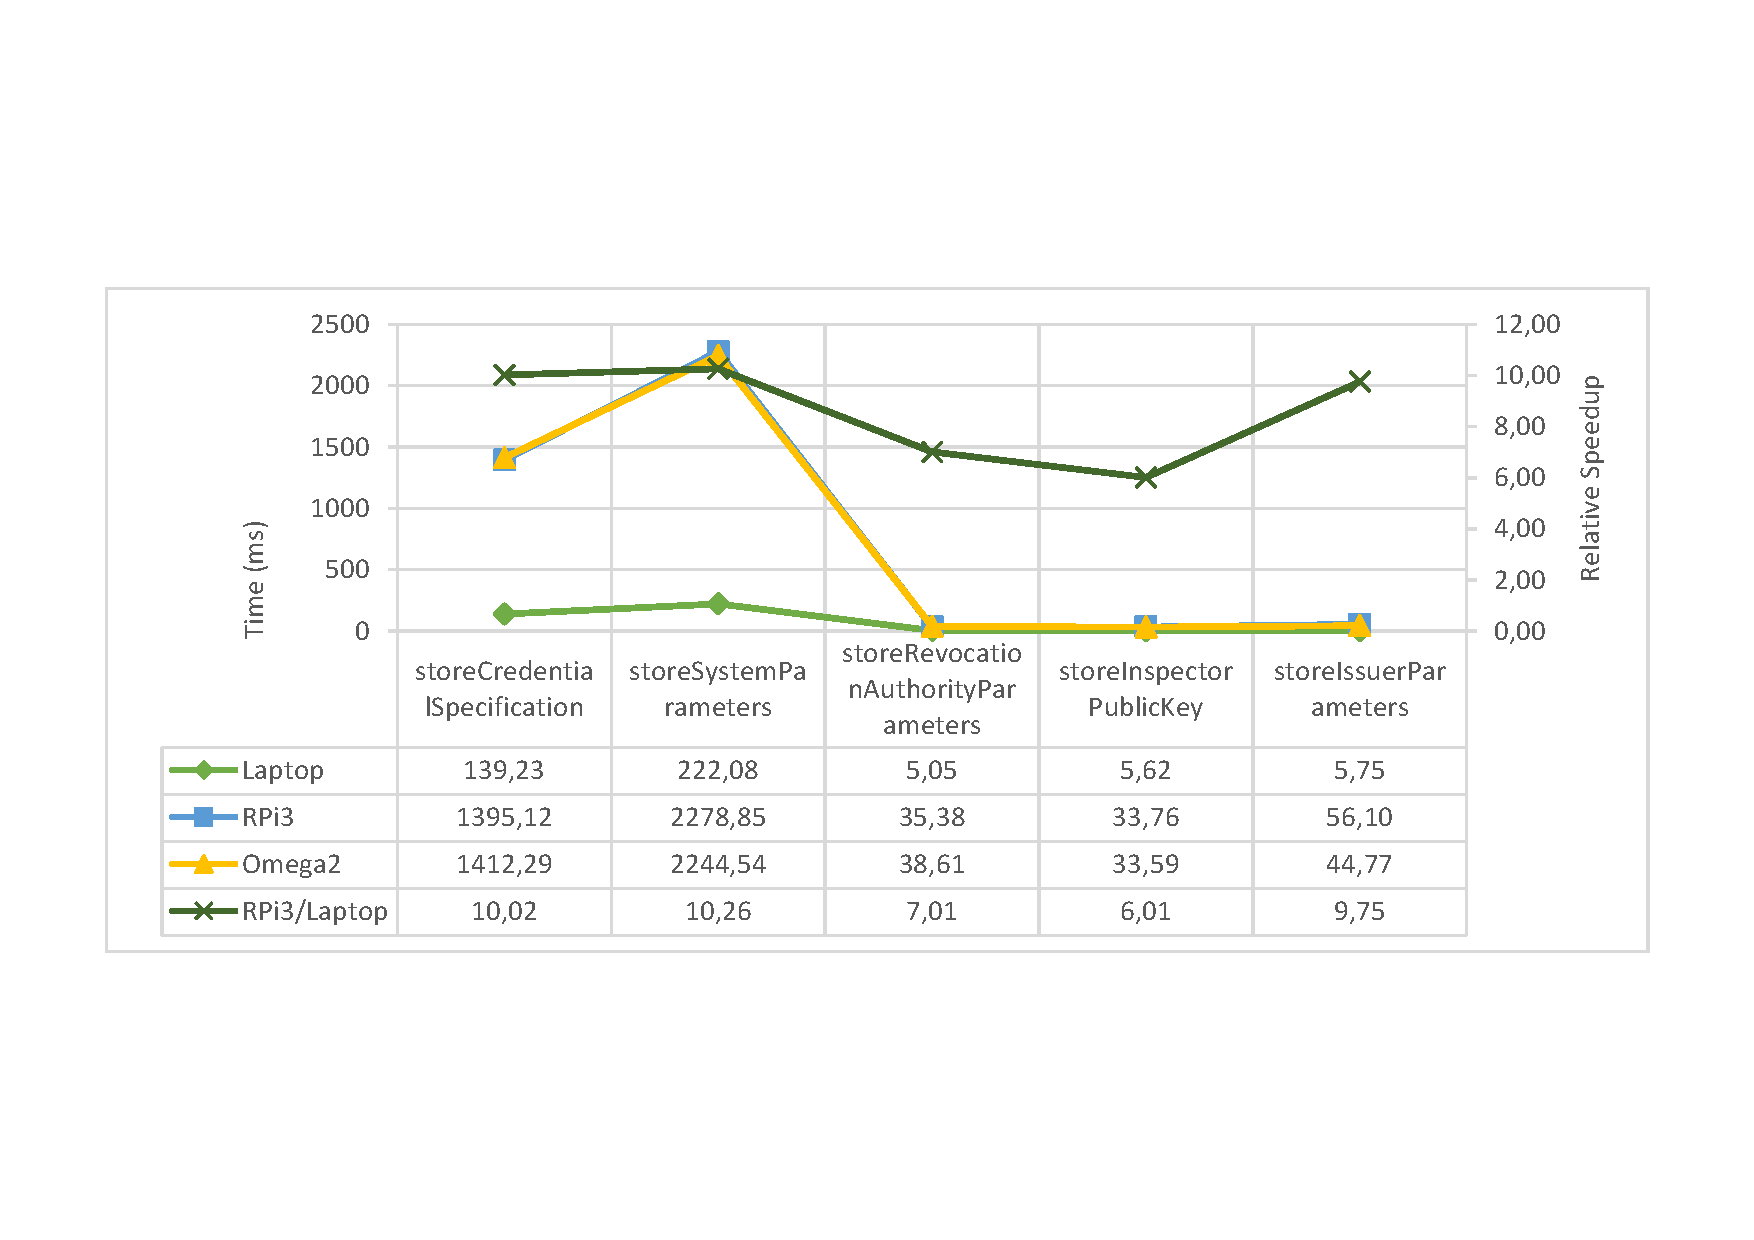
\includegraphics[width=\linewidth]{gfx/graphics/SetupGraphTable}
	\caption{Setup times (milliseconds) and relative speedup.}
	\label{fig:setup:graph}
\end{figure}

%\begin{figure}[bth]
%	\caption{Setup times (milliseconds). Comparison graph}
%	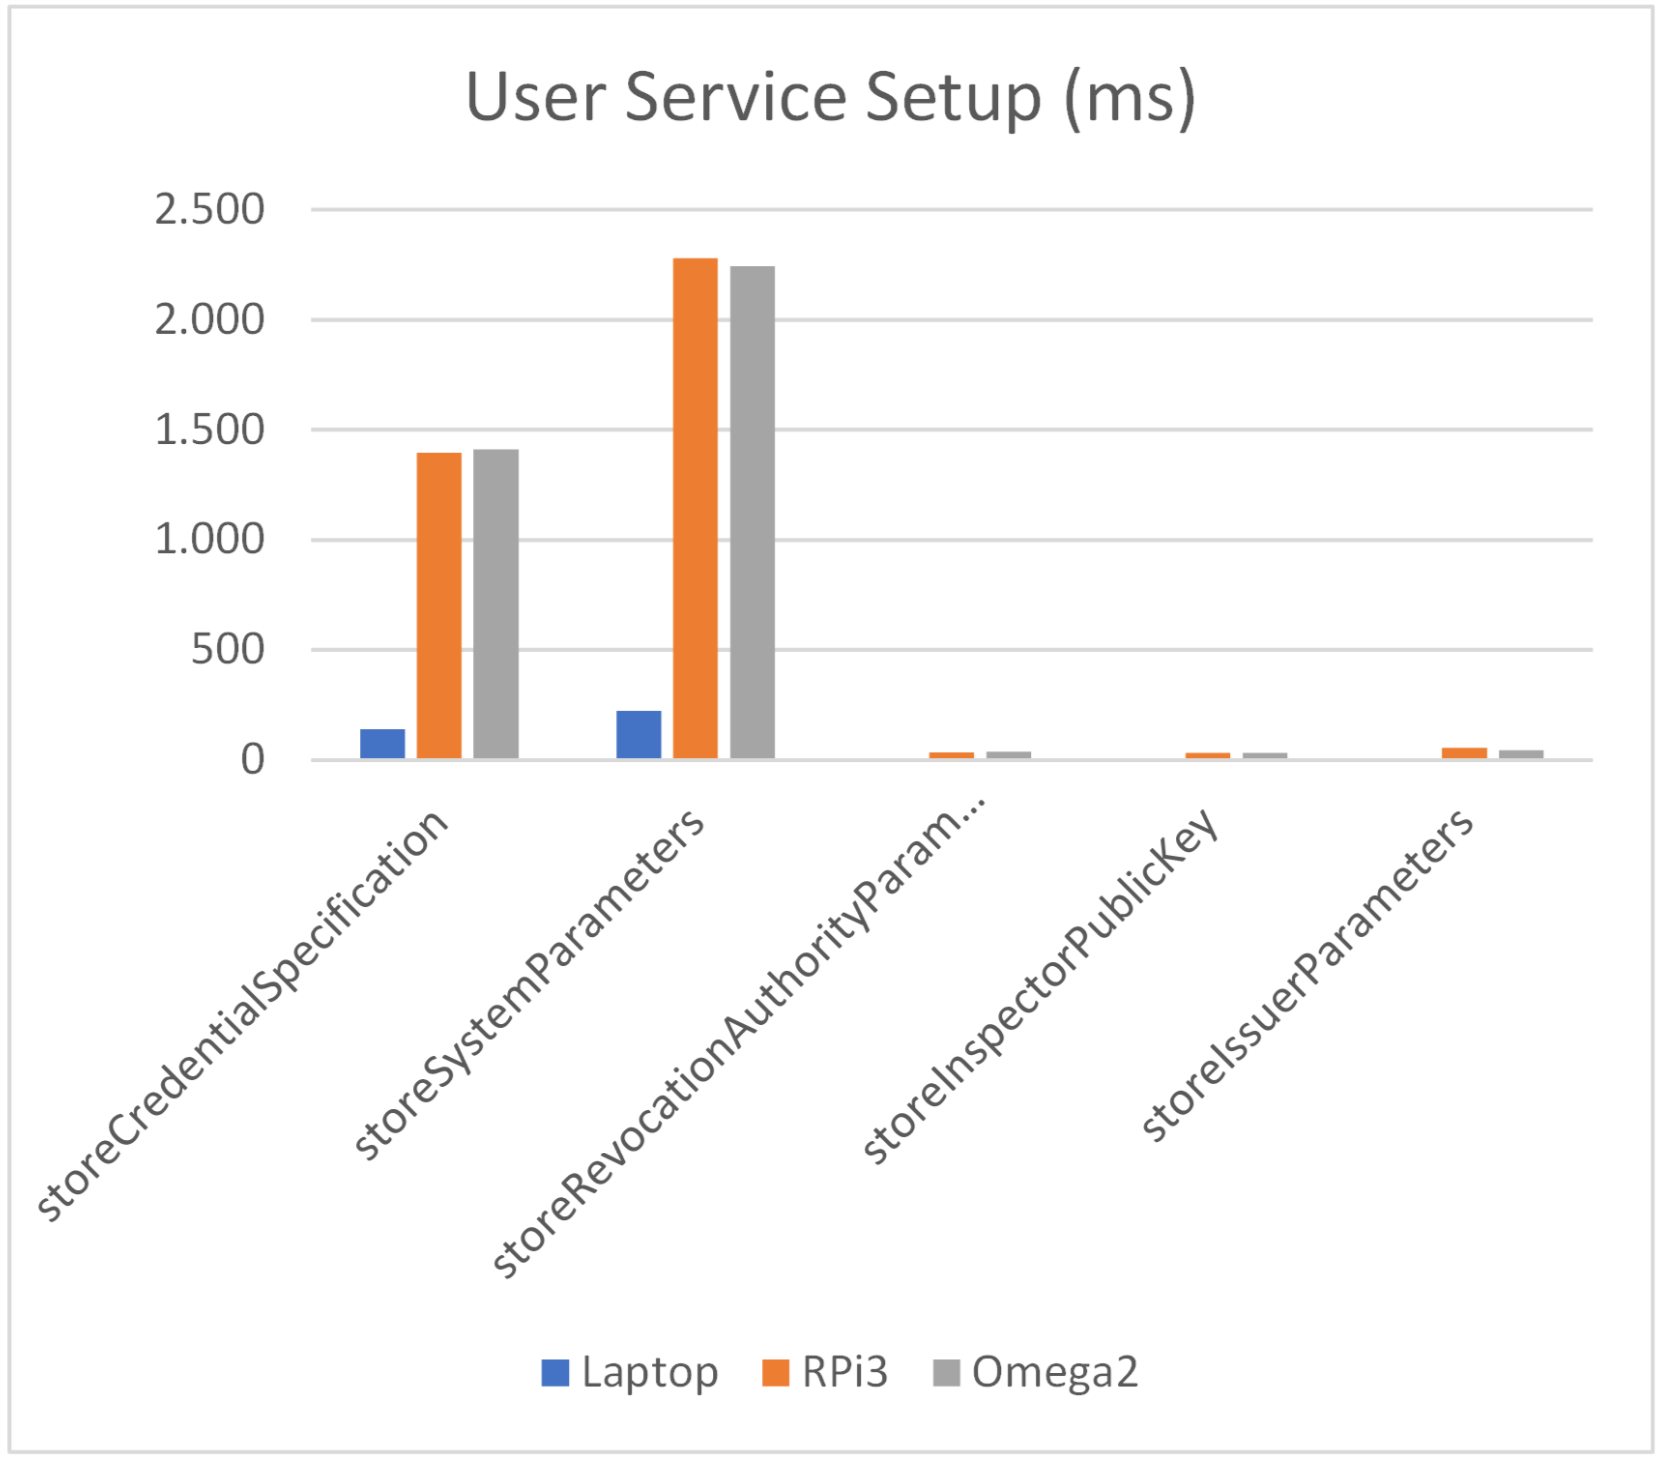
\includegraphics[width=0.8\linewidth]{gfx/graphics/setup}
%	\label{fig:setup:graph2}
%\end{figure}



%\paragraph{Creation of the smart card}\hfil
\hfil

The creation of a \texttt{SoftwareSmartcard} or a \texttt{HardwareSmartcard}, which actually uses the \texttt{IoT Smart Card}, differ in how the hardware version must copy to an external device the cryptographic information of the system, shared during the setup phase, as well as common smart card functionality, like the PIN, PUK, operation mode, etc. Figure~\ref{fig:createSmartCard:graph} shows this difference between the software versions of the laptop and RPi3, and the IoT version. This is a one time procedure per device.


\begin{figure}[bth]
	\begin{center} 
	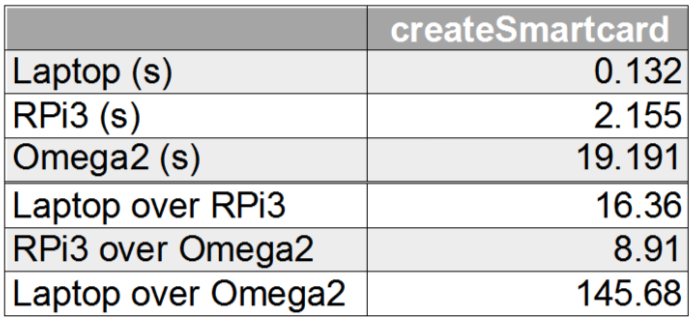
\includegraphics[width=0.5\linewidth]{gfx/graphics/createSCtable}
	\end{center} 
	%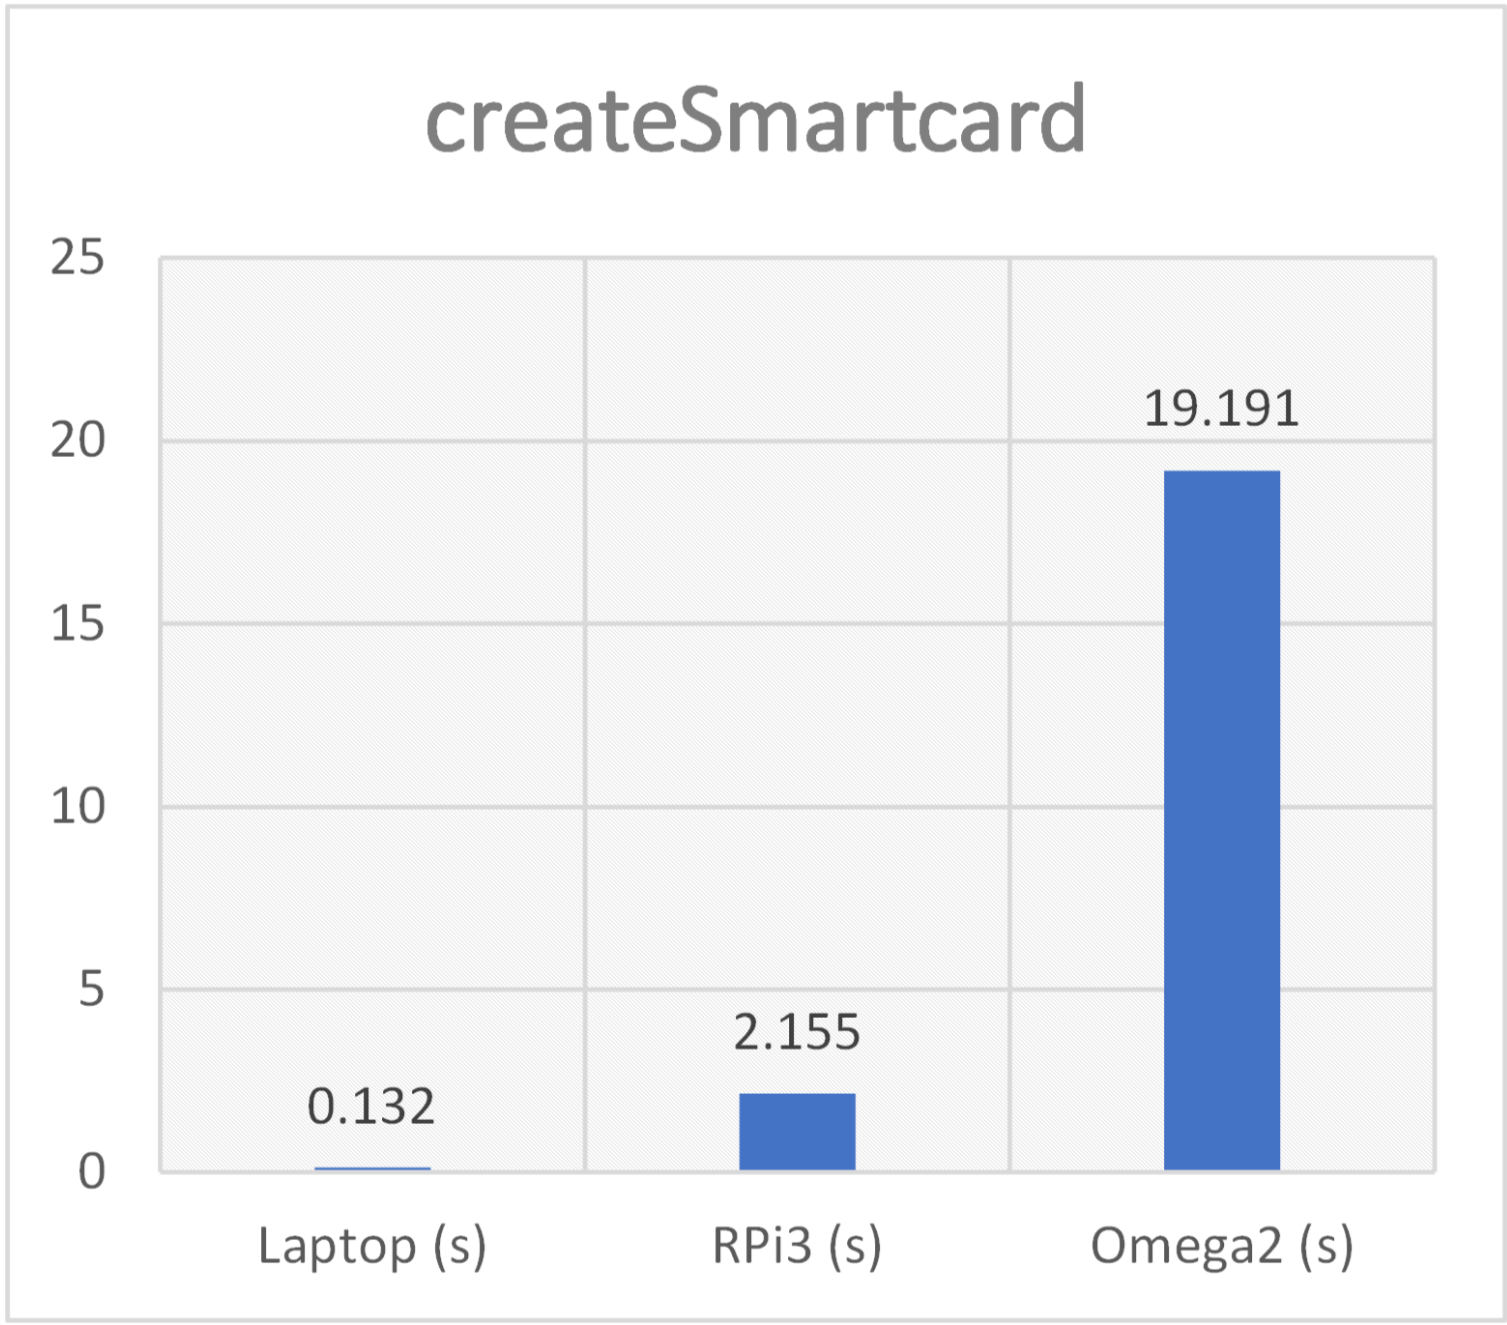
\includegraphics[width=0.4\linewidth]{gfx/graphics/createSC}} 
	\caption{Create smart card times (seconds) and relative speedups.} 
	\label{fig:createSmartCard:graph} 
\end{figure}


%\begin{figure}[bth]
%	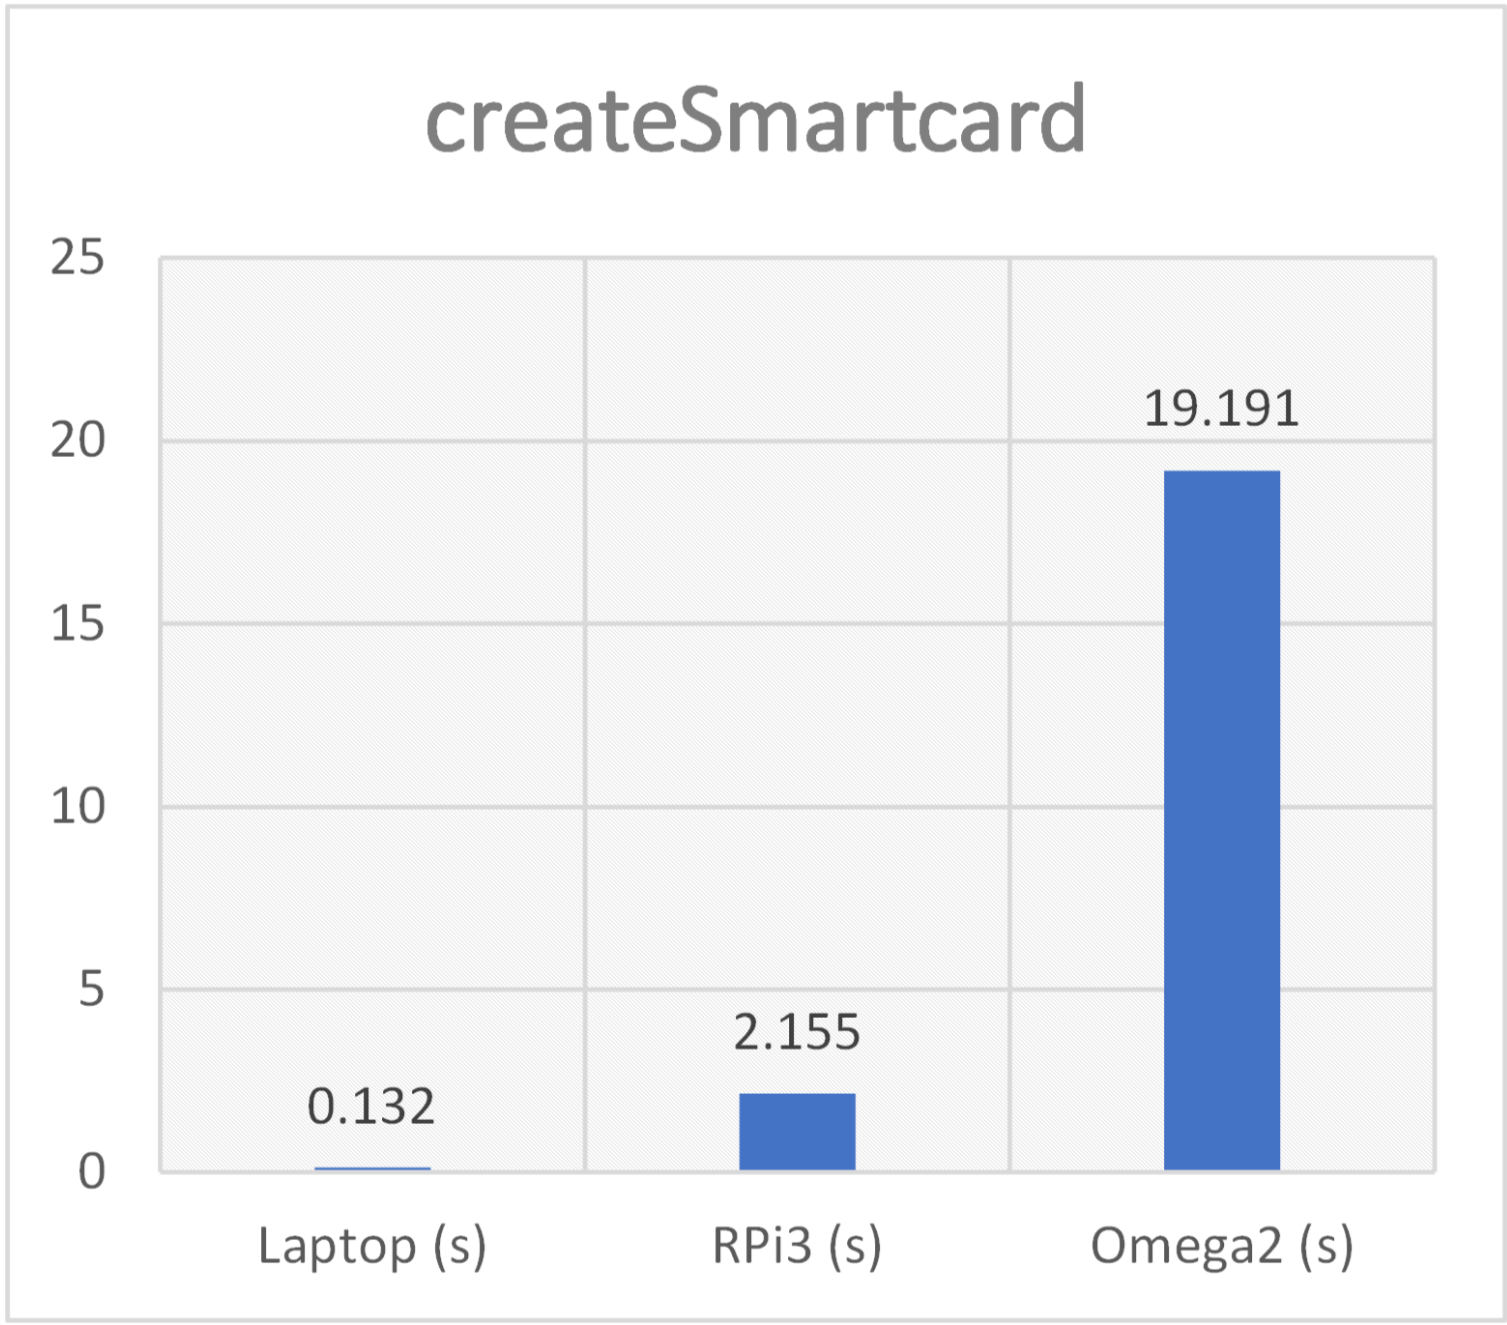
\includegraphics[width=0.8\linewidth]{gfx/graphics/createSC}
%	\caption{Create smart card times (seconds). Comparison graph}
%	\label{fig:createSmartCard:graph2}
%\end{figure}

As this is the first interaction between the RPi3 and the IoT smart card running in the Omega2, it is interesting to analyse the possible network delays. The process uses $30$ APDU Commands, and their respective Responses, with a total of $1109$ bytes. From our network benchmark, the delay in the transmission is around 15 and 20 ms, negligible compared to the total operation time.


%\paragraph{Issuance of the credential}\hfil
\hfil

Next comes the issuance step of the credential with  5 attributes and key sizes of 1024 bits. The process is performed with three REST calls to the User Service, corresponding to the multi-step Idemix credential issuance and identity to use selection. Figure~\ref{fig:issuance:graph} shows the times for each call in each device. The increase of time from the RPi3 to the Omega2 case highlights the difference of processing power between the devices, where the first one makes use of the Java implemented smart card, and the Omega 2 runs the IoT PoC smart card.



%The three delegation steps and the REST method called are:
%
%\begin{itemize}
%	\item First issuance protocol step:\\\texttt{/issuanceProtocolStep}
%	\item Second issuance protocol step (end of first step for the User): \texttt{/issuanceProtocolStepUi}
%	\item Third issuance protocol step (second step for the User): \texttt{/issuanceProtocolStep}
%\end{itemize}



%\begin{figure}[bth]
%	\begin{center}
%		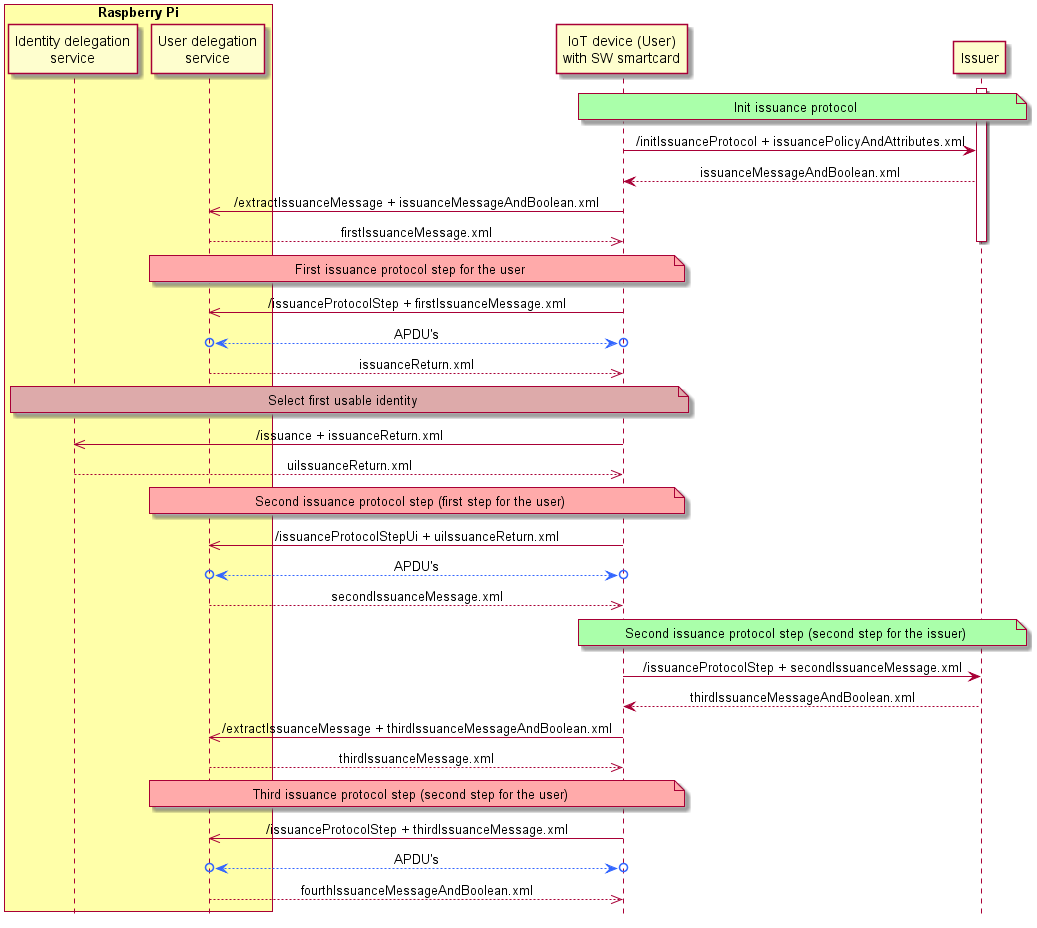
\includegraphics[width=\linewidth]{gfx/UML/IssuanceInteraction}
%	\end{center}
%	\caption{Issuance interaction.}
%	\label{fig:IssuanceInteraction}
%\end{figure}



The three REST calls to the delegation service involved APDU Dialogues with the IoT smart card, with $45$ APDU Commands in total, $3197$ bytes exchanged, that would have introduced a latency of only 45ms from the network.


\begin{figure}[bth]
	\begin{center}
		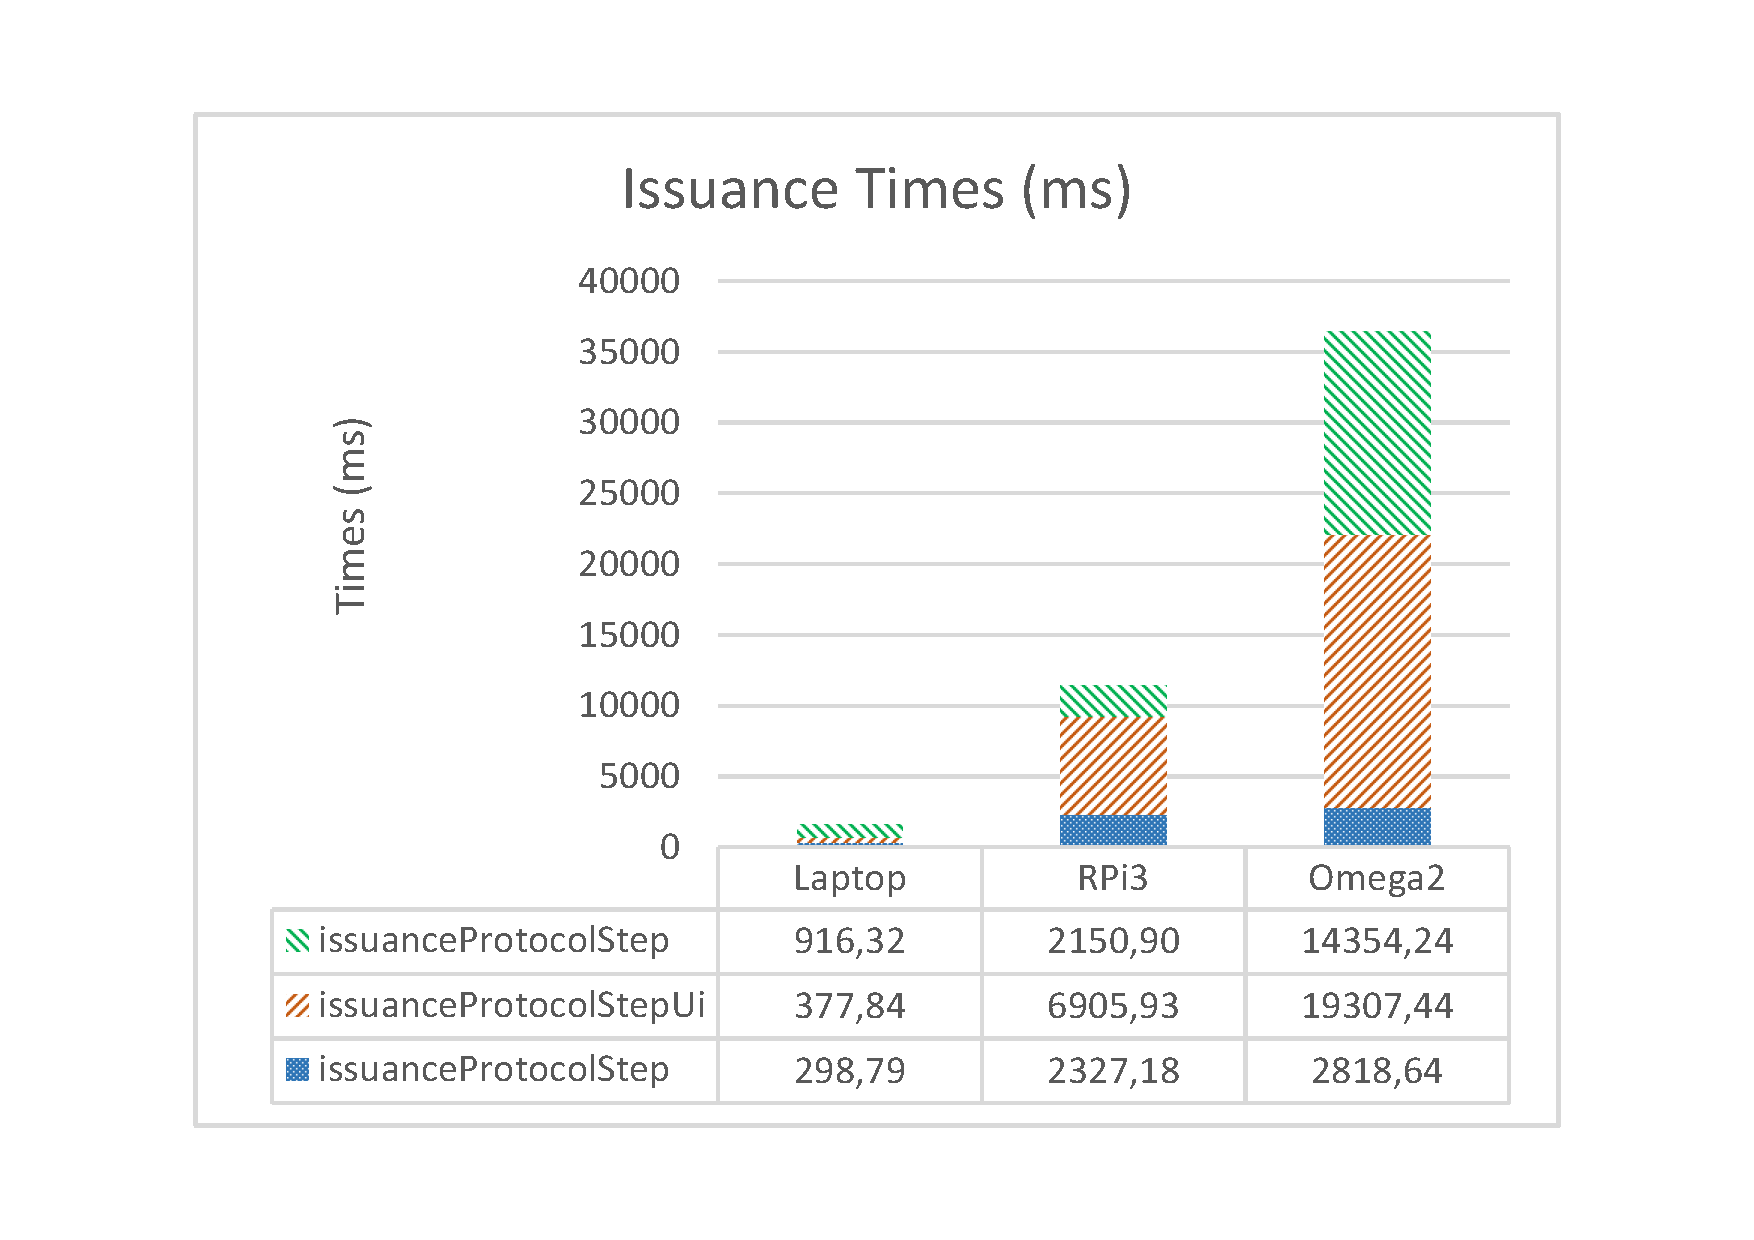
\includegraphics[width=0.8\linewidth]{gfx/graphics/IssuanceGraphTable}
	\end{center}
	\caption{Issuance times (milliseconds)}% and relative speedup.}
	\label{fig:issuance:graph}
\end{figure}

%\begin{figure}[bth]
%	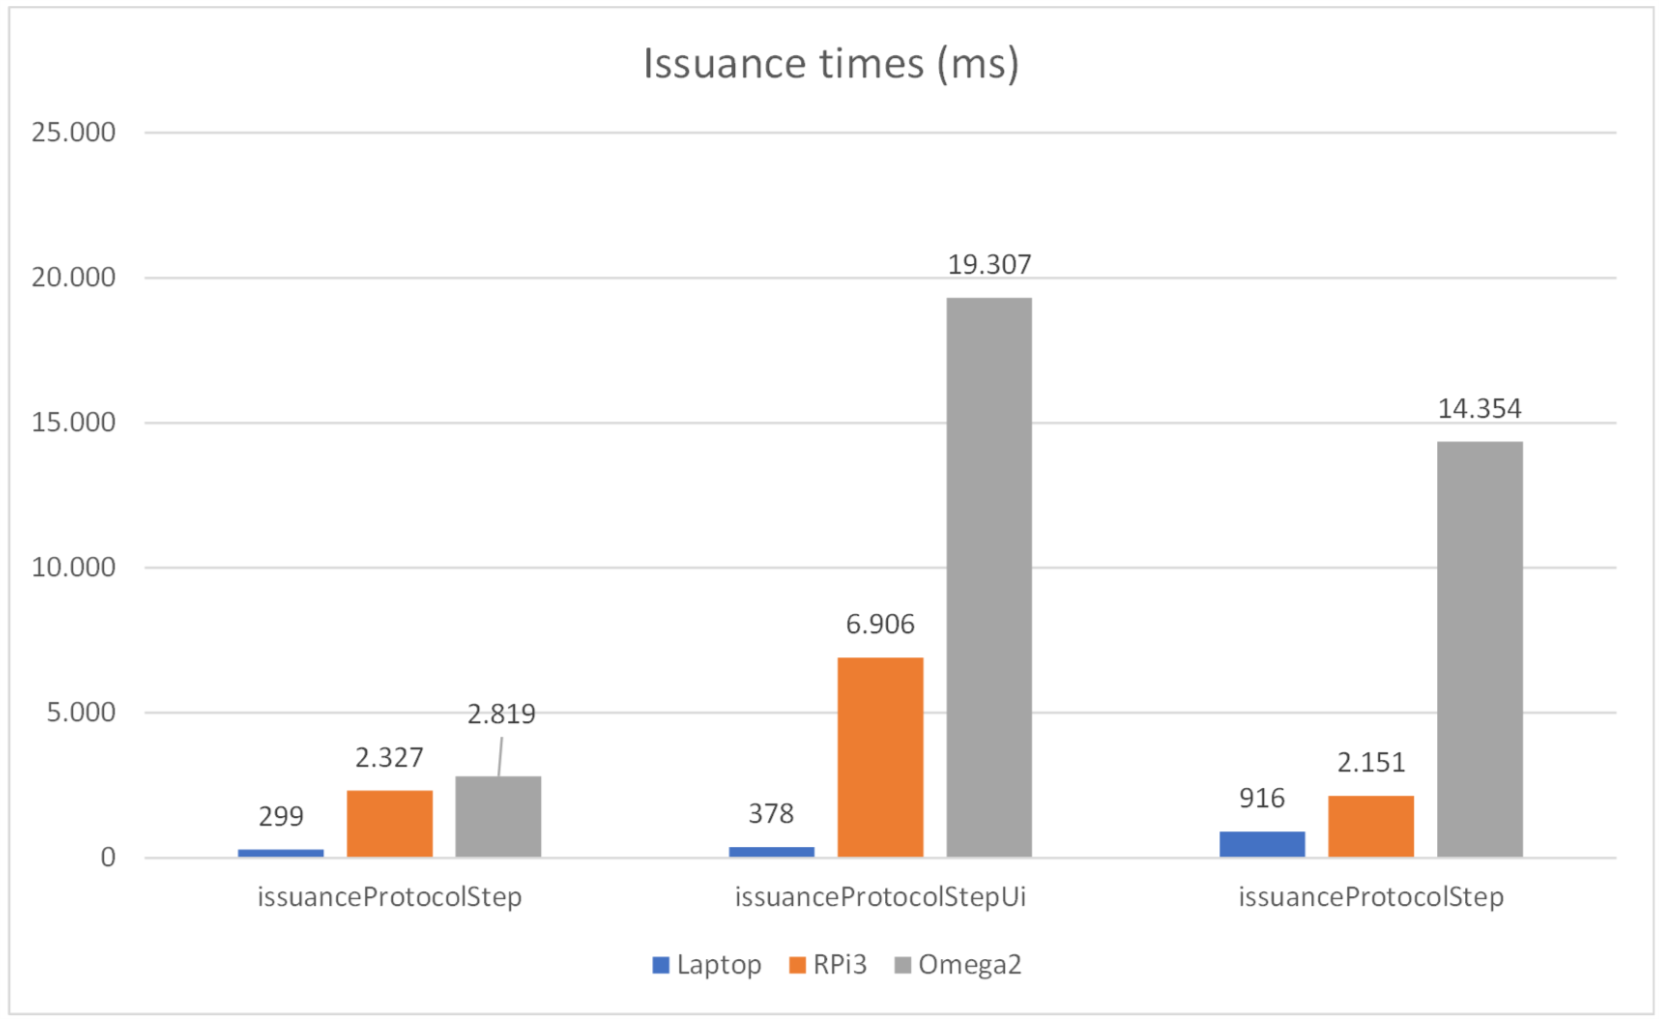
\includegraphics[width=\linewidth]{gfx/graphics/issuance}
%	\caption{Issuance times (milliseconds). Comparison graph}
%	\label{fig:issuance:graph2}
%\end{figure}



%\paragraph{Presentation token}\hfil
\hfil

The final step of the test involves a Proving or Presentation in P2ABCE, where the Verifier sends the User a Presentation Policy, and the User answers with the Presentation Token, without more steps from the User. To ensure that all the process was successful, it was enough to check from the Verifier and the Inspector perspectives that every Token generated was valid.

%\begin{figure}[bth]
%	\begin{center}
%		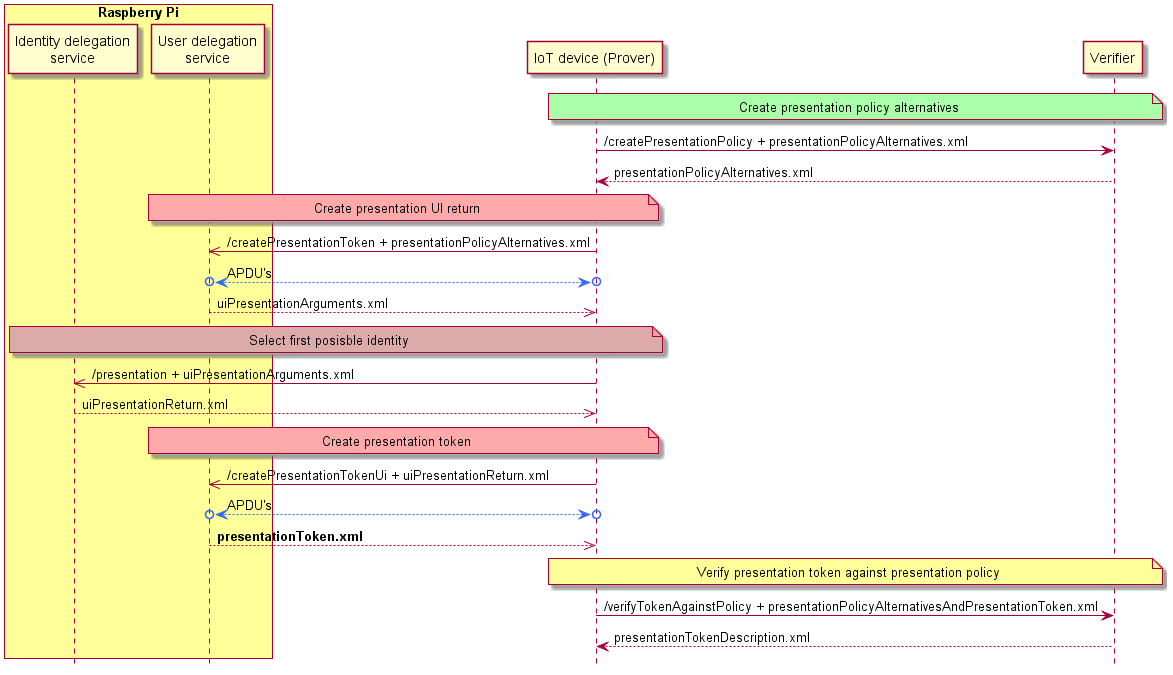
\includegraphics[width=\linewidth]{gfx/UML/ProvingInteraction}
%	\end{center}
%	\caption{Proving interaction.}
%	\label{fig:ProvingInteraction}
%\end{figure}

As shown in Fig.~\ref{fig:proving:graph}, there is a correlation between the cryptographic work the IoT smart card must perform, and the increase of time measured from the RPi3 to the Omega2 cases. 
The APDU Dialogue involved $28$ APDUs, with $1939$ bytes, about only $27$ms of delay from the network.

%The $20$ APDU Commands in the first call make the IoT deployment almost $8$ times slower than the Raspberry Pi 3; but with only $8$ APDU Commands, the second one is less than $1.5$ times slower.

%Nonetheless, it's significant the difference in performance between the laptop and the Raspberry Pi 3 in the last REST call, more than $40$ times slower, even using the \textit{SoftwareSmartcard} in the RPi3.


\begin{figure}[bth]
	\begin{center}
		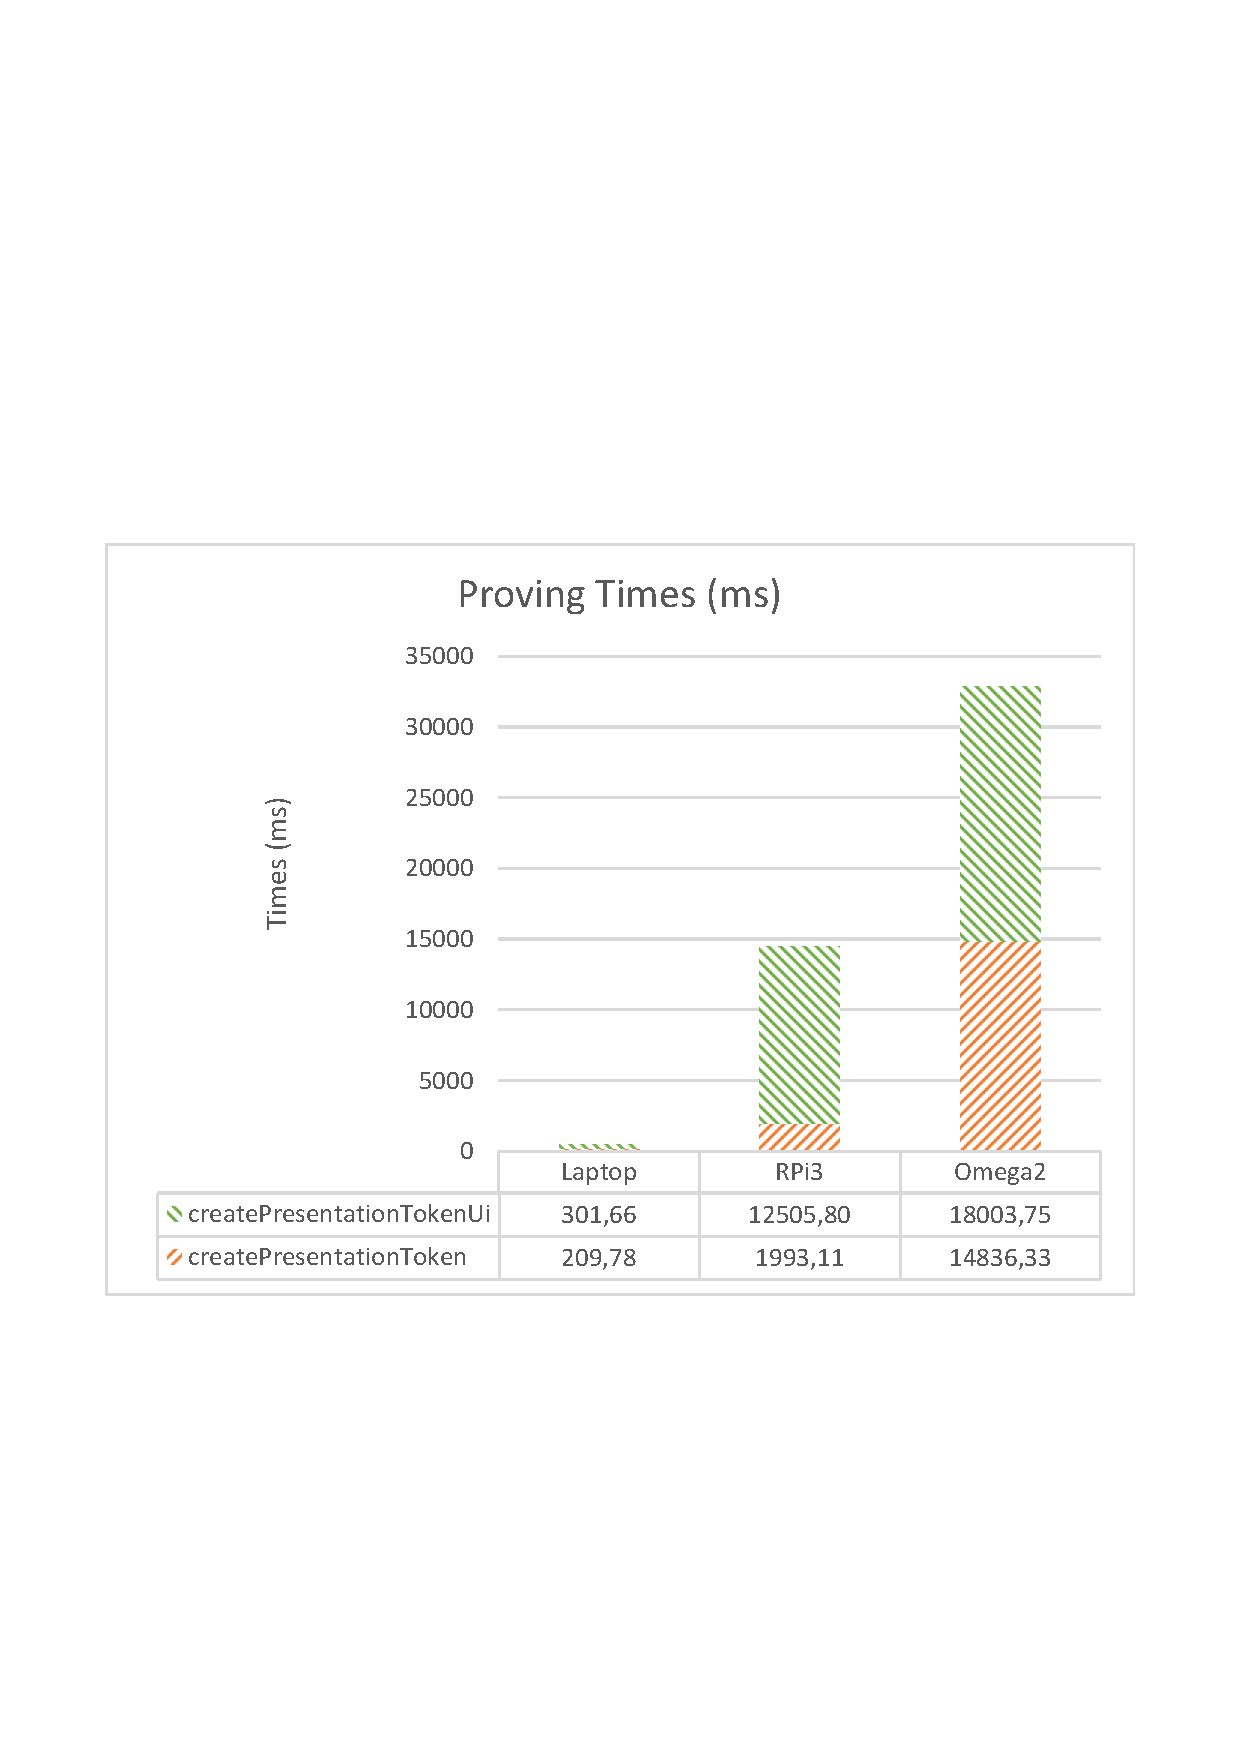
\includegraphics[width=0.8\linewidth]{gfx/graphics/ProvingGraphTable}
	\end{center}
	\caption{Proving times (milliseconds)}% and relative speedup.}
	\label{fig:proving:graph}
\end{figure}

%\begin{figure}[bth]
%	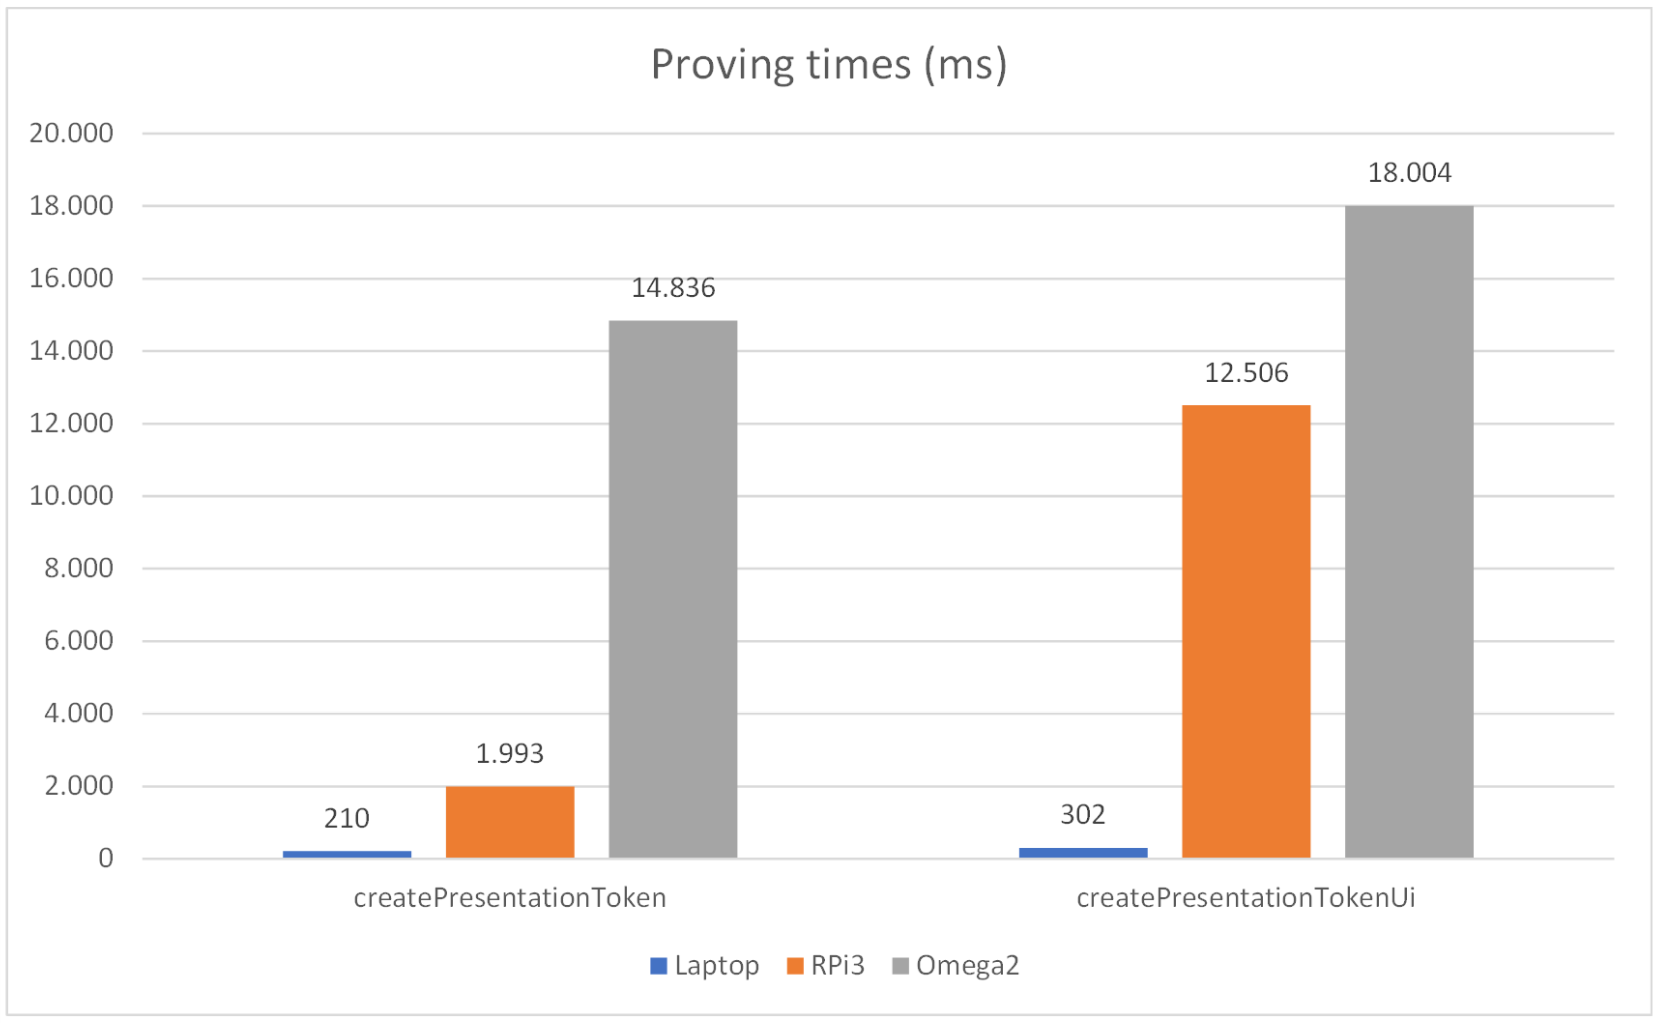
\includegraphics[width=\linewidth]{gfx/graphics/proving}
%	\caption{Proving times (milliseconds). Comparison graph}
%	\label{fig:proving:graph2}
%\end{figure}

Unlike the previous steps, the Proving is the most used method and key feature of the P2ABCE ecosystem. The laptop performs a prove in less than one second, the RPi3 standalone needs $15$ seconds, but our P2ABCE IoT deployment needs $15$ seconds for the first step, and $18$s for the second step, $33$ seconds total to generate a Presentation Token.




\hfil

%\paragraph{Memory usage on the Omega2}\hfil

After the tests, in a new series of executions, the tool \texttt{time -v} provided the \texttt{Maximum resident set size (kbytes)} of the process, i.e. the maximum size of RAM used by the process since its launch. The mean of the maximum memory usage measured was $6569.6$ kbytes. For the IoT smart card this involves the use of static memory for all the \textit{global variables} of the smart card logic, as well as the dynamic memory allocated by the external utilities libraries, like GMPlib, OpenSSL and cJSON.

GMP and OpenSSL always allocate the data in their own ADT, which involves copying the arrays of bytes representing the big modular integers from the cryptographic operations instead of using the byte array representations of the existing smart card logic. cJSON, used in the serialization of the smart card for storage, and debugging purposes, stores a copy of every saved variable in the JSON tree structure, then allocates a string with the JSON, that the user can then write to the save file.

It is important to understand the many bad usages of memory done in this PoC by auxiliary libraries for future improvements of the code. A custom modular library using the same number representations as the smart card logic, an optimized binary serialization method, and many other improvements, are part of our future work.


\subsection{Validation conclusions}

% De https://abc4trust.eu/download/D4.2%20Final%20Reference%20Implementation.pdf  página 45 discussion, que si la credencial está cacheada se reducen ciertos tiempos, este es el peor caso

Below \autoref{totaltime} sums up the time in seconds used in each step of the test for the Omega2 scenario.

The first step, \textit{System Setup} is done only once when the system is being deployed, and the \textit{IoT Smart Card Setup} only once per device.

Because a device can have more than one credential, the Issuance step is significant when we issue multiple credentials over the device's lifetime. We recall that our tests used a credential with five attributes and key sizes of 1024 bits.

Finally, the Proving step is expected to be the most commonly performed operation. The fact that it lasts over half a minute implies that we should not use this PoC for \textit{real-time} applications yet. Nevertheless, for many other IoT applications, the fact this operation can be performed multiple times per hour, presents an useful tool for privacy.


\begin{table}[!ht]
	\begin{center}
		\begin{tabular}{|r|r|r|r|}
			\hline
			System & IoT Smart  & Issue  & Prove Presen-\\
			Setup & Card Setup & credential & tation Policy\\ \hline
			3.77 s & 19.19 s & 36.48 s & 32.84 s \\ \hline
		\end{tabular}
	\end{center}
	\caption{Total time spent for each step in the Omega2+RPi3 scenario.}
	\label{totaltime}
\end{table}

%\begin{figure}[bth]
%	\begin{center}
%		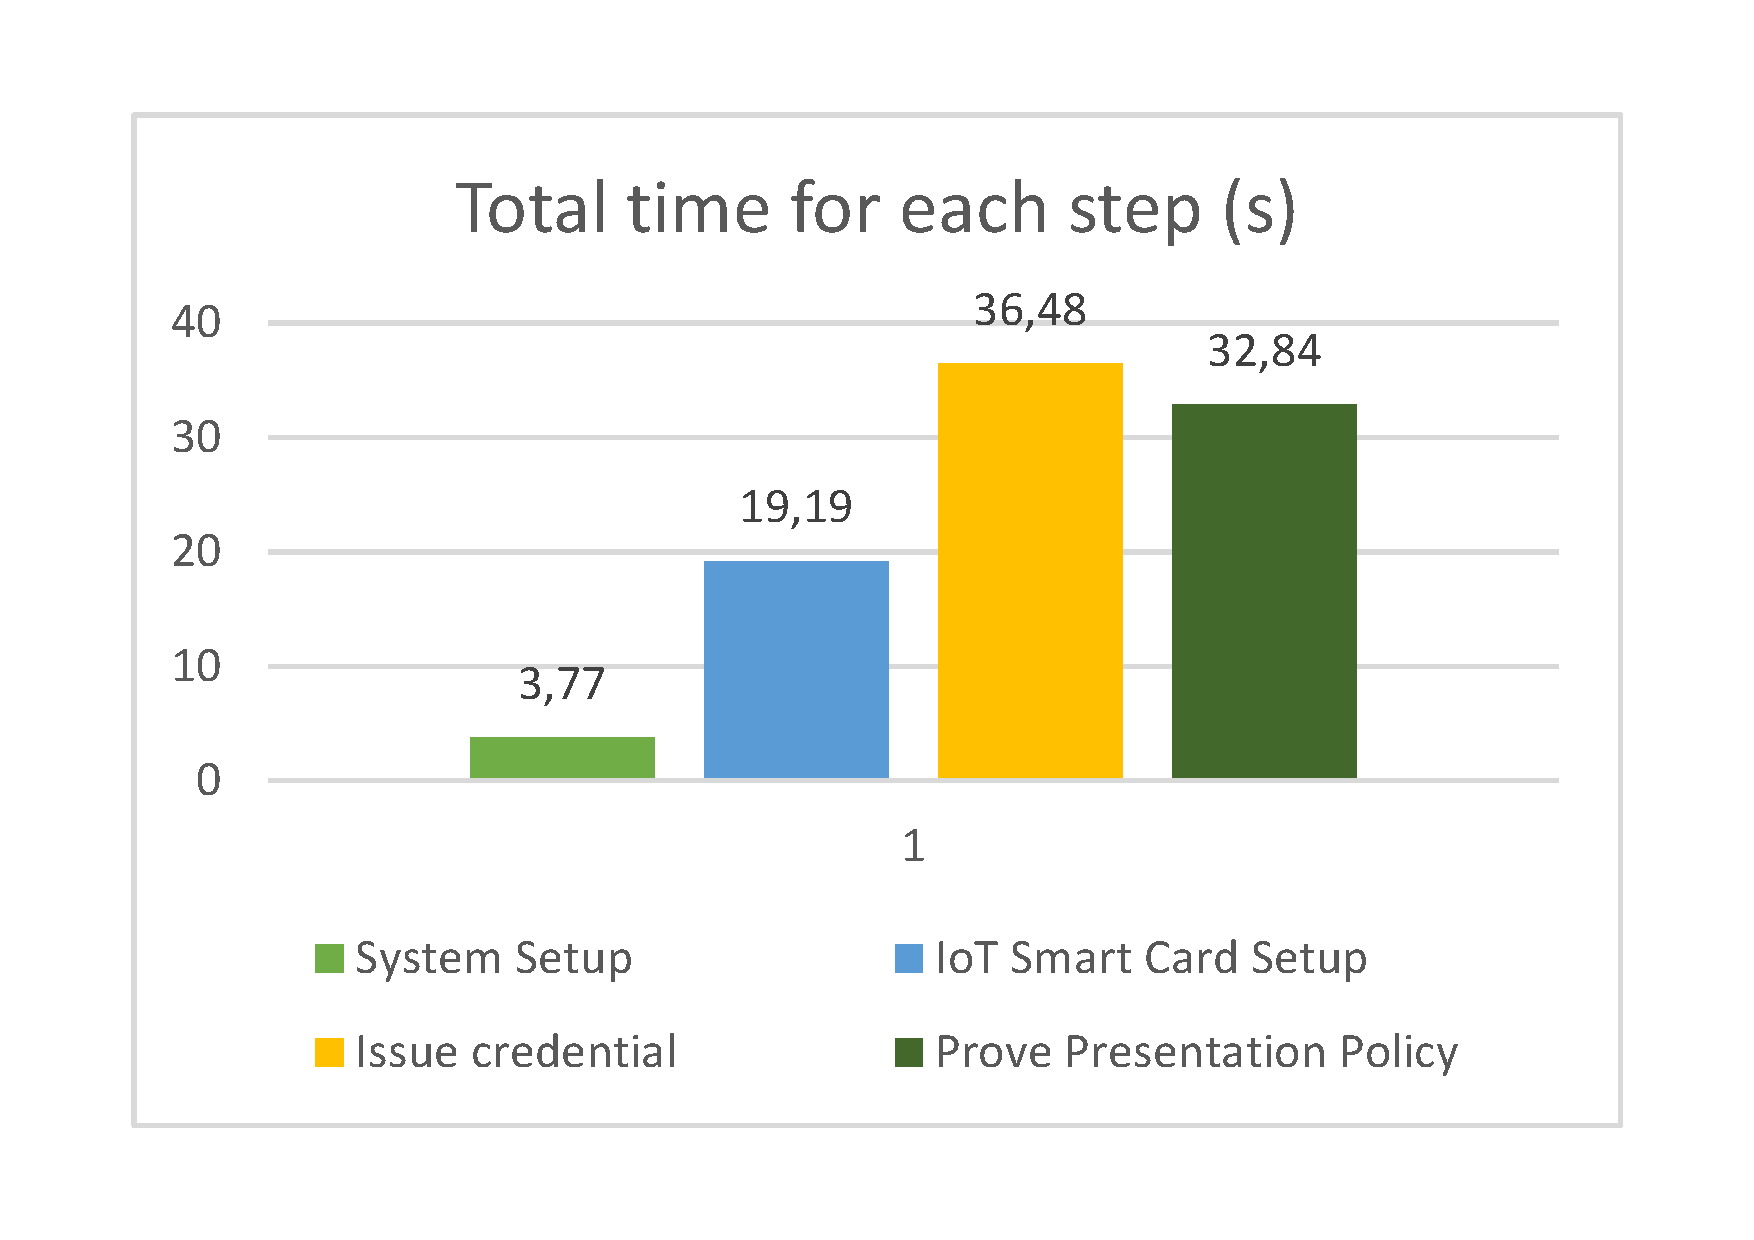
\includegraphics[width=0.75\linewidth]{gfx/graphics/TotalGraph}
%	\end{center}
%	\caption{Total time spent for each step in the Omega2+RPi3 scenario.}
%	\label{totaltime}
%\end{figure}





%************************************************
\section{Conclusions and Future Work}\label{ch:conclusions}
%************************************************

To finish this document, we sum up some conclusions from the work done, and results obtained, as well as some future lines of research.

%\subsection{Conclusions}


In the memory of this project we try to show the work done from the beginning of our research, but we only showed our right decisions, and the information that is significant for the final solution. The truth is that, aside from the information included in this paper, we have worked with other systems that ended up discarded. This isn't a negative aspect, because if we didn't, for example, study the Contiki OS, Cooja simulator and the compatible hardware, we would not be sure the development of a PoC for those systems would be infeasible with the time given.


With regard to the work presented, the flexibility of the computation offloading technique, identifying the key operations that can be delegated, and those ones that can't, has allowed us to define a general solution for the vast world of the Internet of Things. The IoT devices can operate as individual actors in the P2ABCE ecosystem, and when in need of performing computation offloading, the delegation server can also be a device considered into the IoT class.


% Resultados son válidos: feseability, problema de tiempo en sistemas de tiempo real
% Se han conseguido objetivos planteados
% Experiencia: qué era más tedioso, dificultades durante diseño y desarrollo
% Primera aproximación de este tipo ~~: más bien somos el future work de...
% Aplicación de procedimientos aprendidos/aplicados durante el TFG/carrera
% ^ Novelty


During the development, we had to investigate a lot of concepts related to IoT, smart cards, and even the insides of P2ABCE's code, to fix many existing bugs in the original project and minimize the amount of changes it had to undergo, in order to work with the IoT devices.% In the implementation chapter we give guidelines to port MULTOS applications, considering the particularities we encountered, that's why we can't consider it an \textit{instruction manual to port MULTOS apps}, but an interesting reading on how to confront a similar project. For example, if we wanted the Idemix implementation from \cite{vullers2013efficient}, previous to P2ABCE, in a IoT device, we could apply almost the same steps, obtaining a core functionality of Idemix for constrained devices in C.

Our PoC implementation demonstrates that this project is actually feasible, not by performing a simulation of an IoT device, like in \cite{vanet} or \cite{alcaide2013anonymous}, but deploying it in a real IoT device. However, the use of third party non-optimized libraries and no hardware acceleration support, makes the PoC too slow for certain cases, like real-time systems.

%Recalling the objectives listed in \autoref{objectives:section}, we think we accomplish them, except the implementation of a PoC in the most constrained device possible, where we used LEDE to ease our development, and the last objective, where we could have given a use to the PoC, and we leave as part of the future work. In spite of this negative auto-critic, we have to acknowledge that this is the first privacy-preserving ABC implementation for IoT, designed for extensibility, interoperability and maintenance.

%Finally, we are very thankful to IBM's grant for the \textit{Privacy Preserving Identity Management applied to IoT} project, which allowed us to get this far. 


%\subsection{Future work}


%Due to the nature of the project, there exist many options to continue researching in this area.

On the design aspect, we mentioned a P2ABCE API to abstract the delegation process to other processes running in the IoT devices. To develop this API we should study the available solutions to decide how to delegate to the server, e.g. REST, CoAP, RPC, and consider the security issues mentioned in previous sections. Then we can define an standard API and implement it.

%Also, now that an IoT device can perform P2ABCE operations, we could integrate it in a bigger project, like inside an IdM\footnote{Identity Management - KeyRock \url{https://catalogue.fiware.org/enablers/identity-management-keyrock}} system of FIWARE\footnote{\url{https://www.fiware.org/}}, to issue Idemix credentials to both users and IoT devices.% And once the identification is achieved in a privacy-preserving fashion, more applications should be researched, like how the IoT device could benefit from the ZKP cryptography to prove information not issued in its credential, by expanding the P2ABCE presentation policies.


On the implementation side, we would continue with a second PoC which targeted even more constrained devices, like Arduino systems. %Another line of development could be to implement more P2ABCE functionality inside the IoT device, in order to delegate less on the P2ABCE server. 
It also would be interesting to compare the execution of the current PoC to a version with cryptographic hardware acceleration, for example, using Atmel's chips for SHA, AES and secure memory.


%
%\begin{figure}[bth]
%	\begin{center}
%		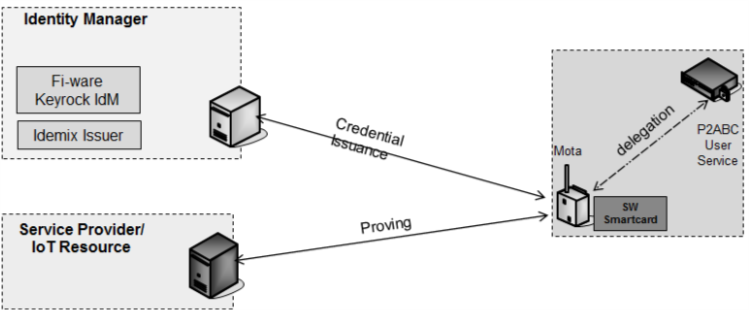
\includegraphics[width=0.8\linewidth]{gfx/fiware}
%		\caption{IoT+Idemix Fi-Ware integration.}
%	\end{center}
%	\label{fig:fiware}
%\end{figure}


\subsection*{Acknowledgements}

The project leading to this application has received funding from IBM 2015 Faculty Award for Cyber Security and the European Union’s Horizon 2020 research and innovation programme under grant agreement No 700085 (ARIES project).



\bibliography{Bibliography}
\bibliographystyle{plain}


\EOD

\end{document}
